%% jan. 4, 2011  items to fix:
%% notation for math and reference to images.
%% how include eps figures.
%% make all the little figures (search for eps) in a common, nice matlab way for the
%% example filtering operations.

\chapter{Image Derivatives}
\label{chapter:image_derivatives}

\section{Introduction}

Computing image derivatives is an essential operator for extracting useful information from images. As we show in the previous chapter, image derivatives allowed us computing boundaries between objects and to have access to some of the three-dimensional (3D) information lost when projecting the 3D world into the camera plane.  Derivatives are useful because they give us information about where are happening the changes in the image and we expect those changes to be correlated with transitions between objects.

%\marginnote{{\bf Notation:} In this chapter we will use both discrete and continuous images. We will denote discrete images as $\img \left[n,m \right]$ and continuous images as $\img (x,y)$.}

The operator that computes the image derivatives a long the spatial dimensions ($x$ and $y$) is a linear system:

\begin{figure}[h]
	\centerline{
	\tikzstyle{int}=[draw, minimum size=3em]
	\tikzstyle{init} = [pin edge={to-,thin,black}]
	\begin{tikzpicture}[node distance=0cm,auto,>=latex']
		\node [int] (box1) {$\left( \frac{\partial}{\partial x}, \frac{\partial}{\partial y} \right)$};
		\node [left of=box1,node distance=2cm] (input) {$\img (x,y)$};
		\node [right of=box1,node distance=2.8cm] (output) {$\left( \img_x(x,y),\img_y(x,y) \right)$};
		\node (c) [right of=box1,node distance=3cm, coordinate] {};
		\path[->] (input) edge node {} (box1);
		\path[->] (box1) edge node {} (output);
	\end{tikzpicture}
	}
	\caption{Computing image derivatives along $x$- and $y$-dimensions.}
	\label{fig:genericfilterH}
\end{figure}

The derivative operator is linear and translation invariant. Therefore, it can be written as a convolution. The following images show an input image and the resulting derivatives along the horizontal and vertical dimensions using one of the discrete approximations that we will discuss in this chapter.

\begin{figure}[h]
	\centerline{
		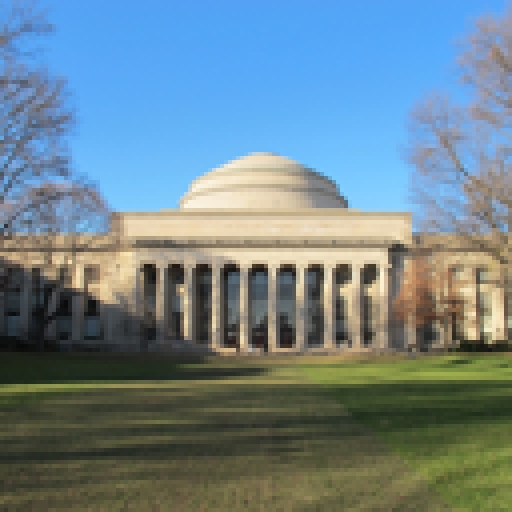
\includegraphics[width=.32\linewidth]{figures/derivatives/mit_der_a.jpg}~
		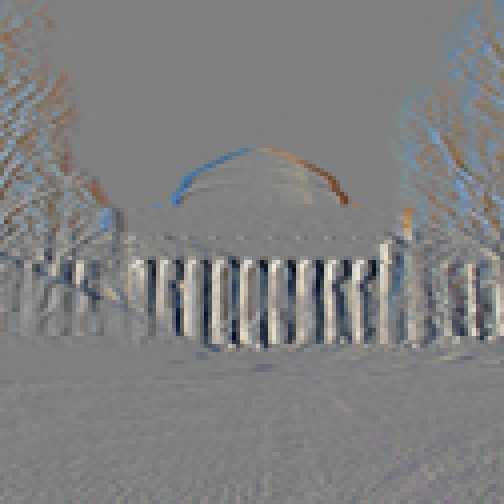
\includegraphics[width=.32\linewidth]{figures/derivatives/mit_der_b.jpg}~
		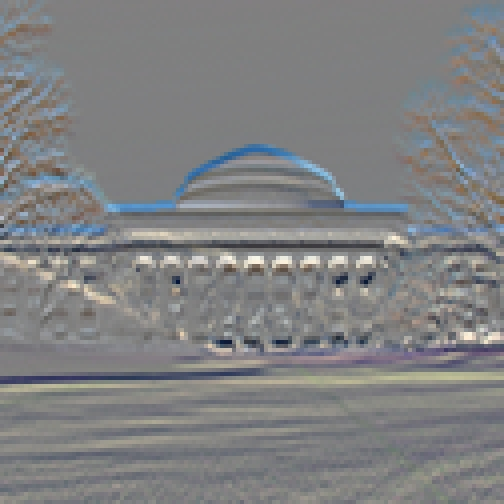
\includegraphics[width=.32\linewidth]{figures/derivatives/mit_der_c.jpg}
		\caption{Image derivatives.
			(left) Input image, (middle) its $x$-derivative, and (right) its $y$-derivative.}
	}
	\label{fig:derivativesmit}
\end{figure}




\section{Discretizing Image Derivatives}

If we had access to the continuous image, then image derivatives could be computed as: $\partial \img (x,y) / \partial x$, which is defined as

\begin{equation}
	\frac{\partial \img(x,y)} {\partial x} = \lim_{\epsilon \to 0} \frac{ \img(x+\epsilon,y) -\img(x,y)} {\epsilon}
\end{equation}

However, there are several reasons why we might not be able to apply this definition:
\begin{itemize}
	\item We only have access to a sampled version of the input image, $\img \left[n,m\right]$, and we can not compute the limit when $\epsilon$ goes to zero.
	\item The image could contains many nonderivable points and the gradient would not be defined. We will see how to address this issue later when we study Gaussian derivatives.
	\item In the presence of noise, the image derivative might not be meaningful as it might just be dominated by the noise and not the by image content.
\end{itemize}

For now, let's focus on the problem of approximating the continuous derivative with discrete operators. As the derivative is a linear operator, it can be approximated by a discrete linear filter. There are several ways in which image derivatives can be approximated.

Let's start with a simple approximation to the derivative operator that we have already played with $d_0  = \left[1, -1 \right]$.
\index{Filter!Derivative}
In one dimension (1D), convolving a signal $\img \left[n \right]$ with this filter results in
\begin{equation}
	\img \circ d_0 = \img \left[n \right] - \img \left[n-1 \right]
\end{equation}
this approximates the derivative by the difference between consecutive values, which is obtained when $\epsilon=1$. \Fig{\ref{fig:discretederivative}}{c} shows the result of filtering a 1D signal (\fig{\ref{fig:discretederivative}}[a]) convolved with $d_0 \left[n\right]$ (\fig{\ref{fig:discretederivative}}[b]). The output is zero wherever the input signal is constant and it is large in the places where there are variations in the input values. However, note that the output is not perfectly aligned with the input. In fact there is half a sample displacement to the right. This is due to the fact that $d_0 \left[n\right]$ is not centered around the origin.

This can be addressed with a different approximation to the spatial derivative $d_1  = \left[1, 0, -1 \right]/2$. In one dimension, convolving a signal $\img \left[n \right]$ with $d_1 \left[n\right]$ results in
\begin{equation}
	\img \circ d_1 = \frac{\img \left[n+1 \right] - \img \left[n-1 \right]}{2}
\end{equation}
\Fig{\ref{fig:discretederivative}}{e} shows the result of filtering the 1D signal (\fig{\ref{fig:discretederivative}}[a]) convolved with $d_1 \left[n\right]$ (\fig{\ref{fig:discretederivative}}[d]). Now the output shows the highest magnitude output in the midpoint where there is variation in the input signal.

\begin{figure}[h]
	\centerline{
		$
			\begin{array}{lcr}
				~ & ~ &
				%\text{(a)}
				\sublabel{a}{
					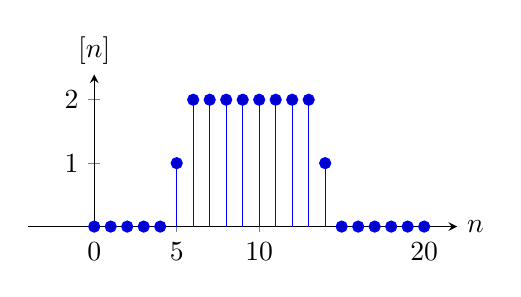
\begin{tikzpicture}
						\begin{axis} [width=200pt,height=100pt,
								axis x line=bottom,
								axis y line=middle,
								tick align=center,
								every axis x label/.style={at={(current axis.right of origin)},anchor=west},
								every axis y label/.style={at={(current axis.above origin)}, anchor=north east,above=0mm},
								xmin=-4, xmax=22,
								xtick={0, 5,10, 20},
								xlabel=$n$,
								ymin=0, ymax=2.4,
								ytick={0,...,2},
								ylabel={$\img \left[n\right]$}]
							\addplot+[ycomb] plot coordinates {(0,0) (1,0) (2,0) (3,0) (4,0) (5,1) (6,2) (7,2) (8,2) (9,2) (10,2) (11,2) (12,2) (13,2) (14,1) (15,0) (16,0) (17,0) (18,0) (19,0) (20,0)};
						\end{axis}
					\end{tikzpicture}
				}
				\\
				%\text{(b)}
				\sublabel{b}{
					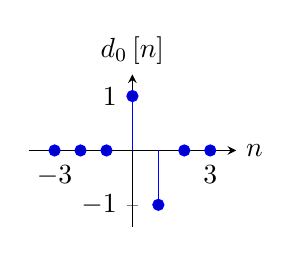
\begin{tikzpicture}
						\begin{axis} [width=120pt,height=100pt,
								axis x line=middle,
								axis y line=middle,
								tick align=center,
								every axis x label/.style={at={(current axis.right of origin)},anchor=west},
								every axis y label/.style={at={(current axis.above origin)}, anchor=north east,above=0mm},
								xmin=-4, xmax=4,
								xtick={-3,3},
								xlabel=$n$,
								ymin=-1.4, ymax=1.4,
								ytick={-1,0,1},
								ylabel={$d_0 \left[n\right]$},
								color=black]
							\addplot+[ycomb] plot coordinates {(-3,0) (-2,0) (-1,0) (0,1) (1,-1) (2,0) (3,0) };
						\end{axis}
					\end{tikzpicture}
				}
				  &
				~
				  &
				\sublabel{c}{
					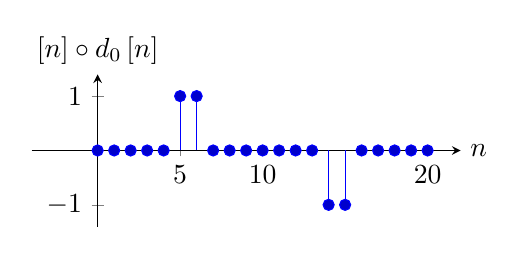
\begin{tikzpicture}
						\begin{axis} [width=200pt,height=100pt,
								axis x line=middle,
								axis y line=middle,
								tick align=center,
								every axis x label/.style={at={(current axis.right of origin)},anchor=west},
								every axis y label/.style={at={(current axis.above origin)}, anchor=north east,above=0mm},
								xmin=-4, xmax=22,
								xtick={0, 5, 10, 20},
								xlabel=$n$,
								ymin=-1.4, ymax=1.4,
								ytick={-1,...,1},
								ylabel={$\img \left[n\right] \circ d_0 \left[n\right]$}]
							%\addplot+[ycomb] plot coordinates {(0,0) (1,0) (2,0) (3,0) (4,0) (5,1) (6,2) (7,2) (8,2) (9,2) (10,2) (11,2) (12,2) (13,2) (14,1) (15,0) (16,0) (17,0) (18,0) (19,0) (20,0)};
							\addplot+[ycomb] plot coordinates {(0,0) (1,0) (2,0) (3,0) (4,0) (5,1) (6,1) (7,0) (8,0) (9,0) (10,0) (11,0) (12,0) (13,0) (14,-1) (15,-1) (16,0) (17,0) (18,0) (19,0) (20,0)};
						\end{axis}
					\end{tikzpicture}
				}
				\\
				\sublabel{d}{
					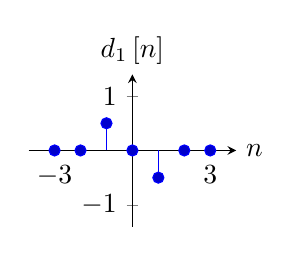
\begin{tikzpicture}
						\begin{axis} [width=120pt,height=100pt,
								axis x line=middle,
								axis y line=middle,
								tick align=center,
								every axis x label/.style={at={(current axis.right of origin)},anchor=west},
								every axis y label/.style={at={(current axis.above origin)}, anchor=north east,above=0mm},
								xmin=-4, xmax=4,
								xtick={-3,3},
								xlabel=$n$,
								ymin=-1.4, ymax=1.4,
								ytick={-1,0,1},
								ylabel={$d_1 \left[n\right]$},
								color=black]
							\addplot+[ycomb] plot coordinates {(-3,0) (-2,0) (-1,1/2) (0,0) (1,-1/2) (2,0) (3,0) };
						\end{axis}
					\end{tikzpicture}
				}
				  &
				~
				  &
				\sublabel{e}{
					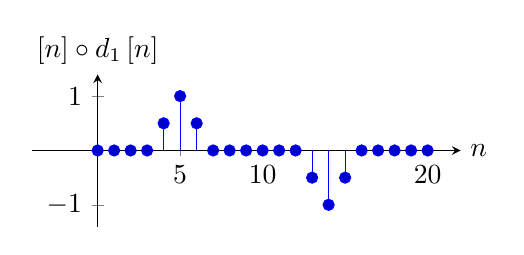
\begin{tikzpicture}
						\begin{axis} [width=200pt,height=100pt,
								axis x line=middle,
								axis y line=middle,
								tick align=center,
								every axis x label/.style={at={(current axis.right of origin)},anchor=west},
								every axis y label/.style={at={(current axis.above origin)}, anchor=north east,above=0mm},
								xmin=-4, xmax=22,
								xtick={0, 5,10, 20},
								xlabel=$n$,
								ymin=-1.4, ymax=1.4,
								ytick={-1,...,1},
								ylabel={$\img \left[n\right] \circ d_1 \left[n\right]$}]
							%\addplot+[ycomb] plot coordinates {(0,0) (1,0) (2,0) (3,0) (4,0) (5,1) (6,2) (7,2) (8,2) (9,2) (10,2) (11,2) (12,2) (13,2) (14,1) (15,0) (16,0) (17,0) (18,0) (19,0) (20,0)};
							\addplot+[ycomb] plot coordinates {(0,0) (1,0) (2,0) (3,0) (4,1/2) (5,1) (6,1/2) (7,0) (8,0) (9,0) (10,0) (11,0) (12,0) (13,-1/2) (14,-1) (15,-1/2) (16,0) (17,0) (18,0) (19,0) (20,0)};
						\end{axis}
					\end{tikzpicture}
				}
			\end{array}
		$
	}
	\caption{(a) Input signal, $\img [n]$. (b) Convolutional kernel $d_0 [n]$, defined as $d_0 [0]=1$ and $d_0 [1]=-1$ and zero everywhere else. (c) Output of the convolution between $\img [n]$ and $d_0 [n]$. (d) Kernel $d_1 [n]$, defined as $d_1 [-1]=1$ and $d_1 [1]=-1$ and zero everywhere else. (e) Output of the convolution between $\img [n]$ and $d_1 [n]$.
	}
	\label{fig:discretederivative}
\end{figure}

It is also interesting to see the behavior of the derivative and its discrete approximations in the Fourier domain. In the continuous domain, the relation ship between the Fourier transform on a function and the Fourier transform of its derivative is
\begin{equation}
	\frac{\partial \img (x)}{\partial x}
	\xrightarrow{\mathscr{F}}
	j w \capitalimg (w)
\end{equation}
In the continuous Fourier domain, derivation is equivalent to multiplying by $jw$. In the discrete domain, the DFT of a signal derivative will depend on the approximation used. Let's study now the DFT of the two approximations that we have discussed here, $d_0$ and $d_1$.

The DFT of $d_0 \left[n\right]$ is
\begin{equation}
	\begin{split}
		D_0 \left[u \right] & = 1 - \exp \left( -2 \pi j \frac{u}{N} \right)                                                                                            \\
		                    & = \exp \left( - \pi j \frac{u}{N} \right) \left(  \exp \left( \pi j \frac{u}{N} \right) - \exp \left( -\pi j \frac{u}{N} \right)  \right) \\
		                    & = \exp \left( - \pi j \frac{u}{N} \right) 2 j \sin (\pi u /N)
	\end{split}
\end{equation}
the first term is a pure phase shift and it is responsible of the half a sample delay in the output. The second term is the amplitude gain and it can be approximated by a linear dependency on $u$ for small $u$ values.

The DFT of $d_1 \left[n\right]$ is
\begin{equation}
	\begin{split}
		D_1 \left[u \right] & =  1/2\exp \left( 2 \pi j \frac{u}{N} \right) - 1/2 \exp \left( -2 \pi j \frac{u}{N} \right) \\
		                    & =  j \sin (2 \pi u /N)
	\end{split}
\end{equation}

\Fig{\ref{fig:d0andd1_dft}} shows the magnitude of $D_0\left[u \right]$ and $D_1\left[u \right]$ and compares it with $\left| 2 \pi u/N \right|$, which will be the ideal approximation to the derivative. The amplitude of $D_0\left[u \right]$ provides a better approximation to the ideal derivative, but the phase of $D_0\left[u \right]$ introduces a small shift in the output. Conversely, $D_1\left[u \right]$ has no shift, but it approximates the derivative over a smaller range of frequencies. The output to $D_1\left[u \right]$ is smoother than the output to $D_0\left[u \right]$, and, in particular, $D_1\left[u \right]$ gives a zero output when the input is the signal $\left[ 1, -1, 1, -1, ... \right]$. In fact, we can see that $\left[1,0,-1\right] = \left[1,-1\right] \circ \left[1,1\right]$, and, therefore $D_1\left[u \right] = D_0\left[u \right] B_1\left[u \right]$, where $B_1\left[u \right]$ is the DFT of the binomial filter $b_1 \left[n \right]$.

\begin{figure}
	\centerline{
		%\begin{center}
		%\[
		%\begin{array}{cc}
		%\text{(a)}
		\sublabel{a}{
			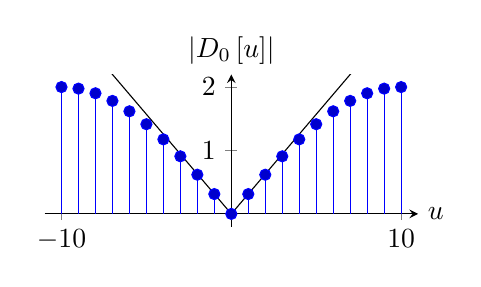
\begin{tikzpicture}
				\begin{axis} [width=180pt,height=100pt,
						axis x line=middle,
						axis y line=middle,
						tick align=center,
						every axis x label/.style={at={(current axis.right of origin)},anchor=west},
						every axis y label/.style={at={(current axis.above origin)}, anchor=north east,above=0mm},
						xmin=-11, xmax=11,
						xtick={-10, 0, 10},
						xlabel=$u$,
						ymin=-0.2, ymax=2.2,
						ytick={0,1,2},
						ylabel={$\left| D_0 \left[ u \right] \right|$}]
					\addplot+[ycomb,domain=-10:10,samples=21,samples y=0]
					({x}, {abs(2*sin(deg(pi*x/20)))});
					\addplot[domain=-10:10,samples=21,samples y=0]
					({x}, {abs(2*pi*x/20)});
				\end{axis}
			\end{tikzpicture}
		}
		%~&~
		%\text{(b)}
		\sublabel{b}{
			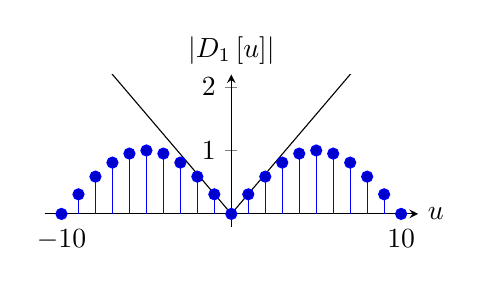
\begin{tikzpicture}
				\begin{axis} [width=180pt,height=100pt,
						axis x line=middle,
						axis y line=middle,
						tick align=center,
						every axis x label/.style={at={(current axis.right of origin)},anchor=west},
						every axis y label/.style={at={(current axis.above origin)}, anchor=north east,above=0mm},
						xmin=-11, xmax=11,
						xtick={-10, 0,10},
						xlabel=$u$,
						ymin=-0.2, ymax=2.2,
						ytick={0,1,2},
						ylabel={$\left| D_1 \left[ u \right] \right|$},
						color=black]
					\addplot+[ycomb,domain=-10:10,samples=21,samples y=0]
					({x}, {abs(sin(deg(2*pi*x/20)))});
					\addplot[domain=-10:10,samples=21,samples y=0]
					({x}, {abs(2*pi*x/20)});
				\end{axis}
			\end{tikzpicture}
		}
		%\end{array}
		%\]
		%\end{center}
	}
	\caption{Magnitude of (a) $D_0\left[u \right]$ and (b) $D_1\left[u \right]$ and comparison with $\left| 2 \pi u/N \right|$, shown as a thin black line. Both DFT are computed over 20 samples.}
	\label{fig:d0andd1_dft}
\end{figure}


When working with two-dimensional (2D) images there are several ways in which partial image derivatives can be approximated. For instance, we can compute derivatives along the $n$ and $m$ components.

\begin{equation}
	\begin{bmatrix}
		1 \\
		-1
	\end{bmatrix}
	~~~~~~~
	\begin{bmatrix}
		1 & -1
	\end{bmatrix}
\end{equation}
The problem with this discretization of the image derivatives is that the outputs are spatially miss-aligned because a filter of length 2 shifts the output image by half a pixel as we discussed earlier. The spatial miss-alignment can be removed by using a slightly different version of the same operator: we can use a rotated reference frame as it is done in the {\bf Roberts cross} operator\index{Roberts cross operator}, introduced in 1963 \cite{Roberts63} in a time when reading an image of $256 \times 256$ pixels into memory took several minutes:
\begin{equation}
	\begin{bmatrix}
		1 & ~0 \\
		0 & -1
	\end{bmatrix}
	~~~~~~~
	\begin{bmatrix}
		~0 & 1 \\
		-1 & 0
	\end{bmatrix}
\end{equation}
Now, both outputs are spatially aligned because they are shifted in the same way. Another discretization is the Sobel operator,
based on the $[-1,0,1]$ kernel, and will be discussed in \sect{\ref{sec:derivatives_binomial_filters}}.

%Although these operators are very old and better algorithms exist nowadays for edge extraction, when an efficient solution is needed, these simple operators are still very useful and had been used as key operators in modern computer vision descriptors such as SIFT \cite{Lowe04},or HOG \cite{Dalal2005}.

While newer algorithms for edge extraction have been developed since the creation of these operators, they still hold value in cases where efficiency is important. These simple operators continue to be used as fundamental components in modern computer vision descriptors, including the Scale-invariant feature transform (SIFT) \cite{Lowe04} and the histogram of oriented gradients (HOG) \cite{Dalal2005}.

\section{Gradient-Based Image Representation}

Derivatives have become an important tool to represent images and they can be used to extract a great deal of information from the image as it was shown in the previous chapter. One thing about derivatives is that it might seem as we are loosing information from the input image. An important question is if we have the derivative of a signal, can we recover the original image? What information is being lost? Intuitively, we should be able to recover the input image by integrating its derivative, but it is an interesting exercise to look in detail how this integration can be performed. We will start with a 1D signal and then we will discuss the 2D case.

A simple way of seeing that we can recover the input from its derivatives is to write the derivative in matrix form. This is the matrix that corresponds to the convolution with the kernel $\left[1, -1 \right]$ that we will call $\mathbf{D_0}$. The next two matrices show the matrix $\mathbf{D_0}$ and its inverse $\mathbf{D_0}^{-1}$ for a 1D image of length five pixels using zero boundary conditions:
\begin{equation}
	\mathbf{D_0} =
	\begin{bmatrix}
		1 ~  & 0 ~  & 0 ~  & 0~   & 0 \\
		-1 ~ & 1 ~  & 0 ~  & 0~   & 0 \\
		0 ~  & -1 ~ & 1 ~  & 0 ~  & 0 \\
		0~   & 0 ~  & -1 ~ & 1 ~  & 0 \\
		0~   & 0 ~  & 0 ~  & -1 ~ & 1
	\end{bmatrix}
	~~~~~~~~~
	\mathbf{D_0}^{-1} =
	\begin{bmatrix}
		1 ~ & ~ 0 ~ & ~ 0 ~ & ~ 0~  & ~ 0 \\
		1 ~ & ~ 1 ~ & ~ 0 ~ & ~ 0~  & ~ 0 \\
		1 ~ & ~ 1 ~ & ~ 1 ~ & ~ 0 ~ & ~ 0 \\
		1~  & ~ 1 ~ & ~ 1 ~ & ~ 1 ~ & ~ 0 \\
		1~  & ~ 1 ~ & ~ 1 ~ & ~ 1 ~ & ~ 1
	\end{bmatrix}
\end{equation}
We can see that the inverse $\mathbf{D_0}^{-1}$ is reconstructing each pixel as a sum of all the derivative values from the left-most pixel to the right.  And the inverse perfectly reconstructs the input. But, this is cheating because the first sample of the derivative gets to see the actual value of the input signal and then we can integrate back the entire signal. That matrix is assuming zero boundary conditions for the signal and the boundary gives us the needed constraint to be able to integrate back the input signal.

But what happens if you only get to see valid differences and you remove any pixel that was affected by the boundary? In this case, the derivative operator in matrix form is
\begin{equation}
	\mathbf{D_0} =
	\begin{bmatrix}
		-1 ~ & 1 ~  & 0 ~  & 0~   & 0 \\
		0 ~  & -1 ~ & 1 ~  & 0 ~  & 0 \\
		0~   & 0 ~  & -1 ~ & 1 ~  & 0 \\
		0~   & 0 ~  & 0 ~  & -1 ~ & 1
	\end{bmatrix}
\end{equation}

Let's consider the next 1D input signal:
\begin{equation}
	\boldimg = \left[1, 1, 2, 2, 0\right]
\end{equation}

Then, the output of the derivative operator is
\begin{equation}
	\mathbf{r}=\mathbf{D_0} \boldimg=\left[0, -1, 0, 2\right]
\end{equation}
Note that this vector has one sample less than the input. To recover the input $\boldimg$ we can not invert $\mathbf{D_0}$ as it is not a square matrix, but we can compute the pseudoinverse which turns out to be
\begin{equation}
	\mathbf{D_0}^{+} = \frac{1}{5}
	\begin{bmatrix}
		-4 ~ & -3 ~ & -2~  & -1 \\
		1 ~  & -3 ~ & -2 ~ & -1 \\
		1~   & 2 ~  & -2 ~ & -1 \\
		1~   & 2 ~  & 3 ~  & -1 \\
		1~   & 2 ~  & 3 ~  & 4
	\end{bmatrix}
\end{equation}
The pseudoinverse has an interesting structure and it is easy to see how it can be written in the general form for signals of length $N$. Also note that $\mathbf{D_0}^{+}$ can not be written as a convolution.
Another important thing is that the inversion process is trying to recover more samples than there are observations. The trade off is that the signal that it will recover will have zero mean (so it looses one degree of freedom that can not be estimated). In this example, the reconstructed input is
\begin{equation}
	\hat{\boldimg} = \mathbf{D_0}^{+} \mathbf{r} =
	\left[-0.2, -0.2, 0.8, 0.8, -1.2 \right]
\end{equation}
Note that $\hat{\boldimg}$ is a zero mean vector. In fact, the recovered input is a shifted version of the original input, $\hat{\boldimg} = \boldimg - 1.2$, where 1.2 is the mean value of samples on $\boldimg$.
Then, you still can recover the input signal up to the DC component (mean signal value).


\section{Image Editing in the Gradient Domain}
\label{section:editinggradientdomain}



One of the interests of transforming an image into a different representation than pixels is that it allows us to manipulate aspects of the image that would be hard to control using the pixels directly. \Fig{\ref{fig:edit_with_derivatives}} shows an example of image editing using derivatives.

\begin{figure}
	\centerline{
		\includegraphics[width=1\linewidth]{figures/derivatives/stop_impainting.eps}
	}
	\caption{Image inpainting: Using image derivatives we delete the word ``stop'' by setting to zero  the gradients indicated by the mask. The resulting decoded image propagates the red color inside the region that contained the word.}
	\label{fig:edit_with_derivatives}
\end{figure}


First, the image is {\bf encoded} using derivatives along the $x$ and $y$ dimensions:
\begin{equation}
	\mathbf{r} =
	\left[
		\begin{array}{c}
			\mathbf{D_x} \\
			\mathbf{D_y}
		\end{array}
		\right]
	\boldimg
\end{equation}
The resulting representation, $\mathbf{r}$, contains the concatenation of the output of  both derivative operators.  $\mathbf{r}$ will have high values in the image regions that contains changes in pixel intensities and colors and will be near zero in regions with small variations. This representation can be {\bf decoded} back into the input image by using the pseudoinverse as we did in the 1D case. The pseudoinverse can be efficiently computed in the Fourier domain \cite{Weiss01derivingintrinsic}.


We can now manipulate this representation. In the example shown in \fig{\ref{fig:edit_with_derivatives}}, if we set to zero the image derivatives that correspond to the word ``stop'', when we decode the representation we obtain a new image where the word ``stop'' has been removed. The red color fills\footnote{{\bf Image inpainting} consists in filling a missing region in an image.}  the region with the word is present in the input image.
We did not have to specify what color that region had to be, that information comes from the integration process. Therefore, deleting an object using image derivatives can be achieved by setting to zero the gradients regardless of the color of the background. Unfortunately, things get more complex when the background has texture and this simple technique will fail.

%Show some applications doing edge edition. This is a non-linear filter.



\section{Gaussian Derivatives}

In the previous sections we studied how to discretize derivatives and how to use them to represent images. However, computing derivatives in practice presents several difficulties. First, derivatives are sensitive to noise. In the presence of noise, as images tend to vary slowly, the difference between two continuous pixel values will be dominated by noise. This is illustrated in \fig{\ref{fig:derivativesnoisystop}}.


\begin{figure}[h]
	\centerline{
		\sublabel{a}{
			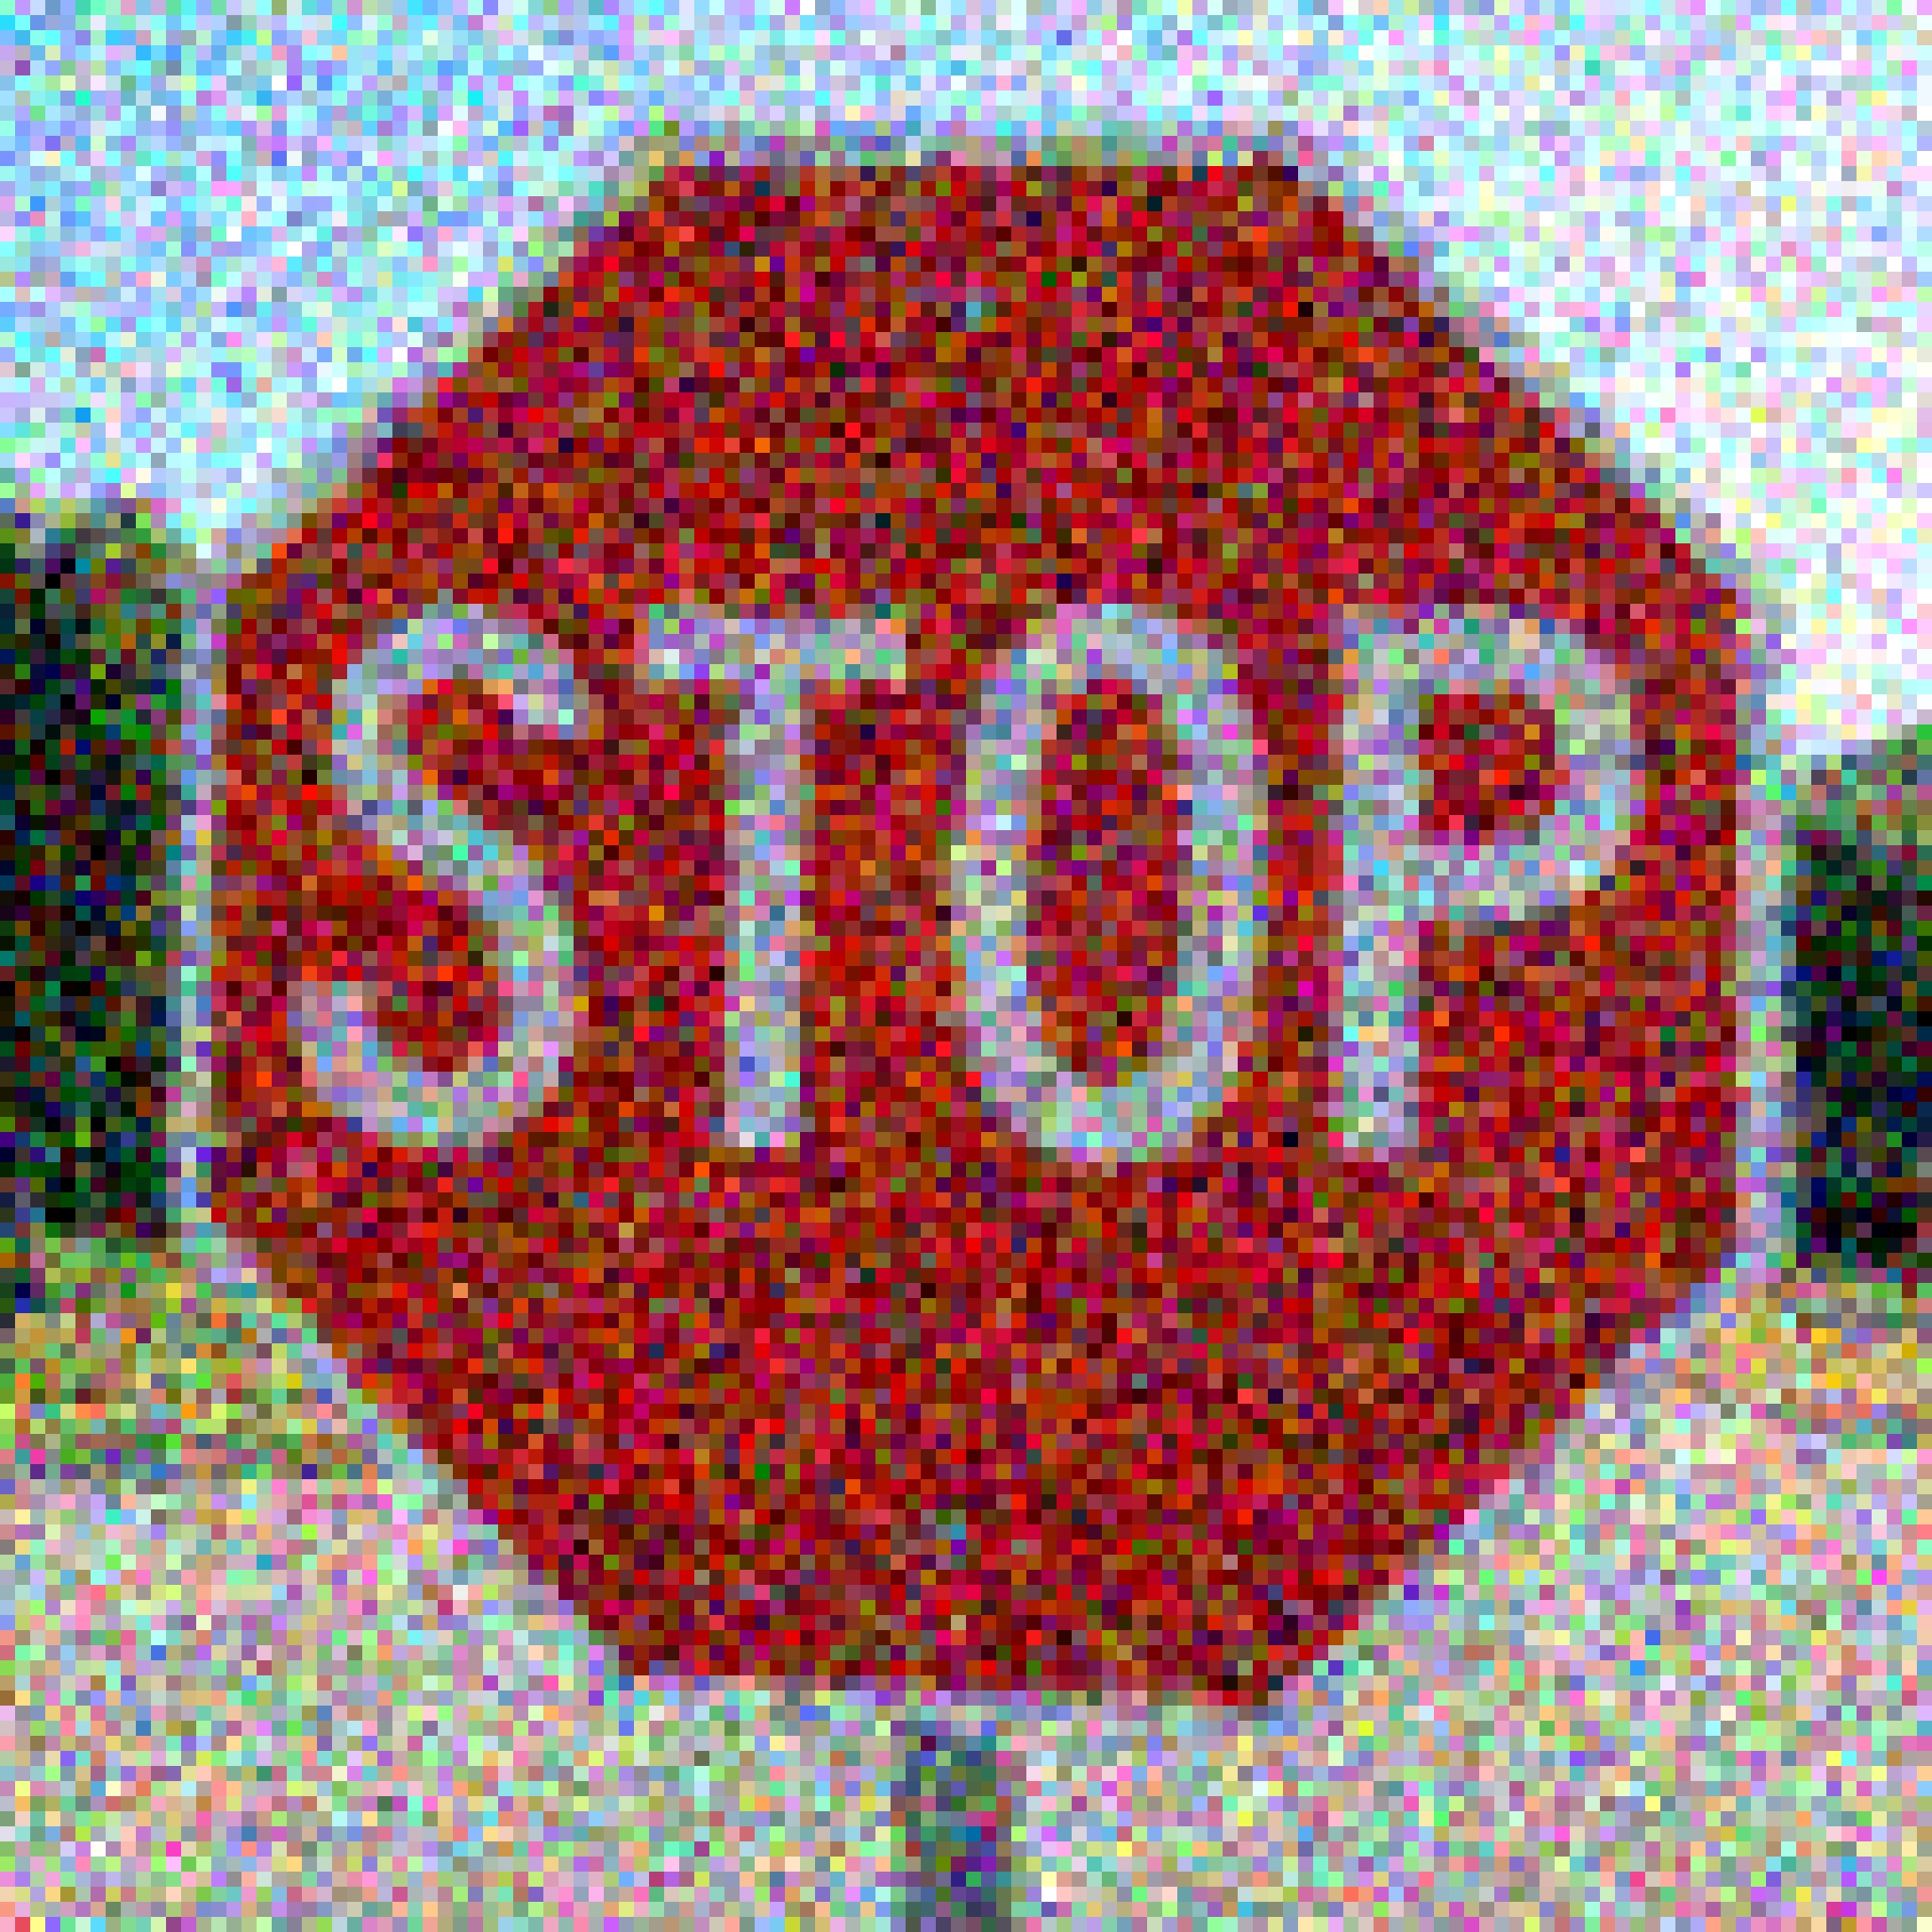
\includegraphics[width=.3\linewidth]{figures/derivatives/stop_noise.jpg}
		}
		\sublabel{b}{
			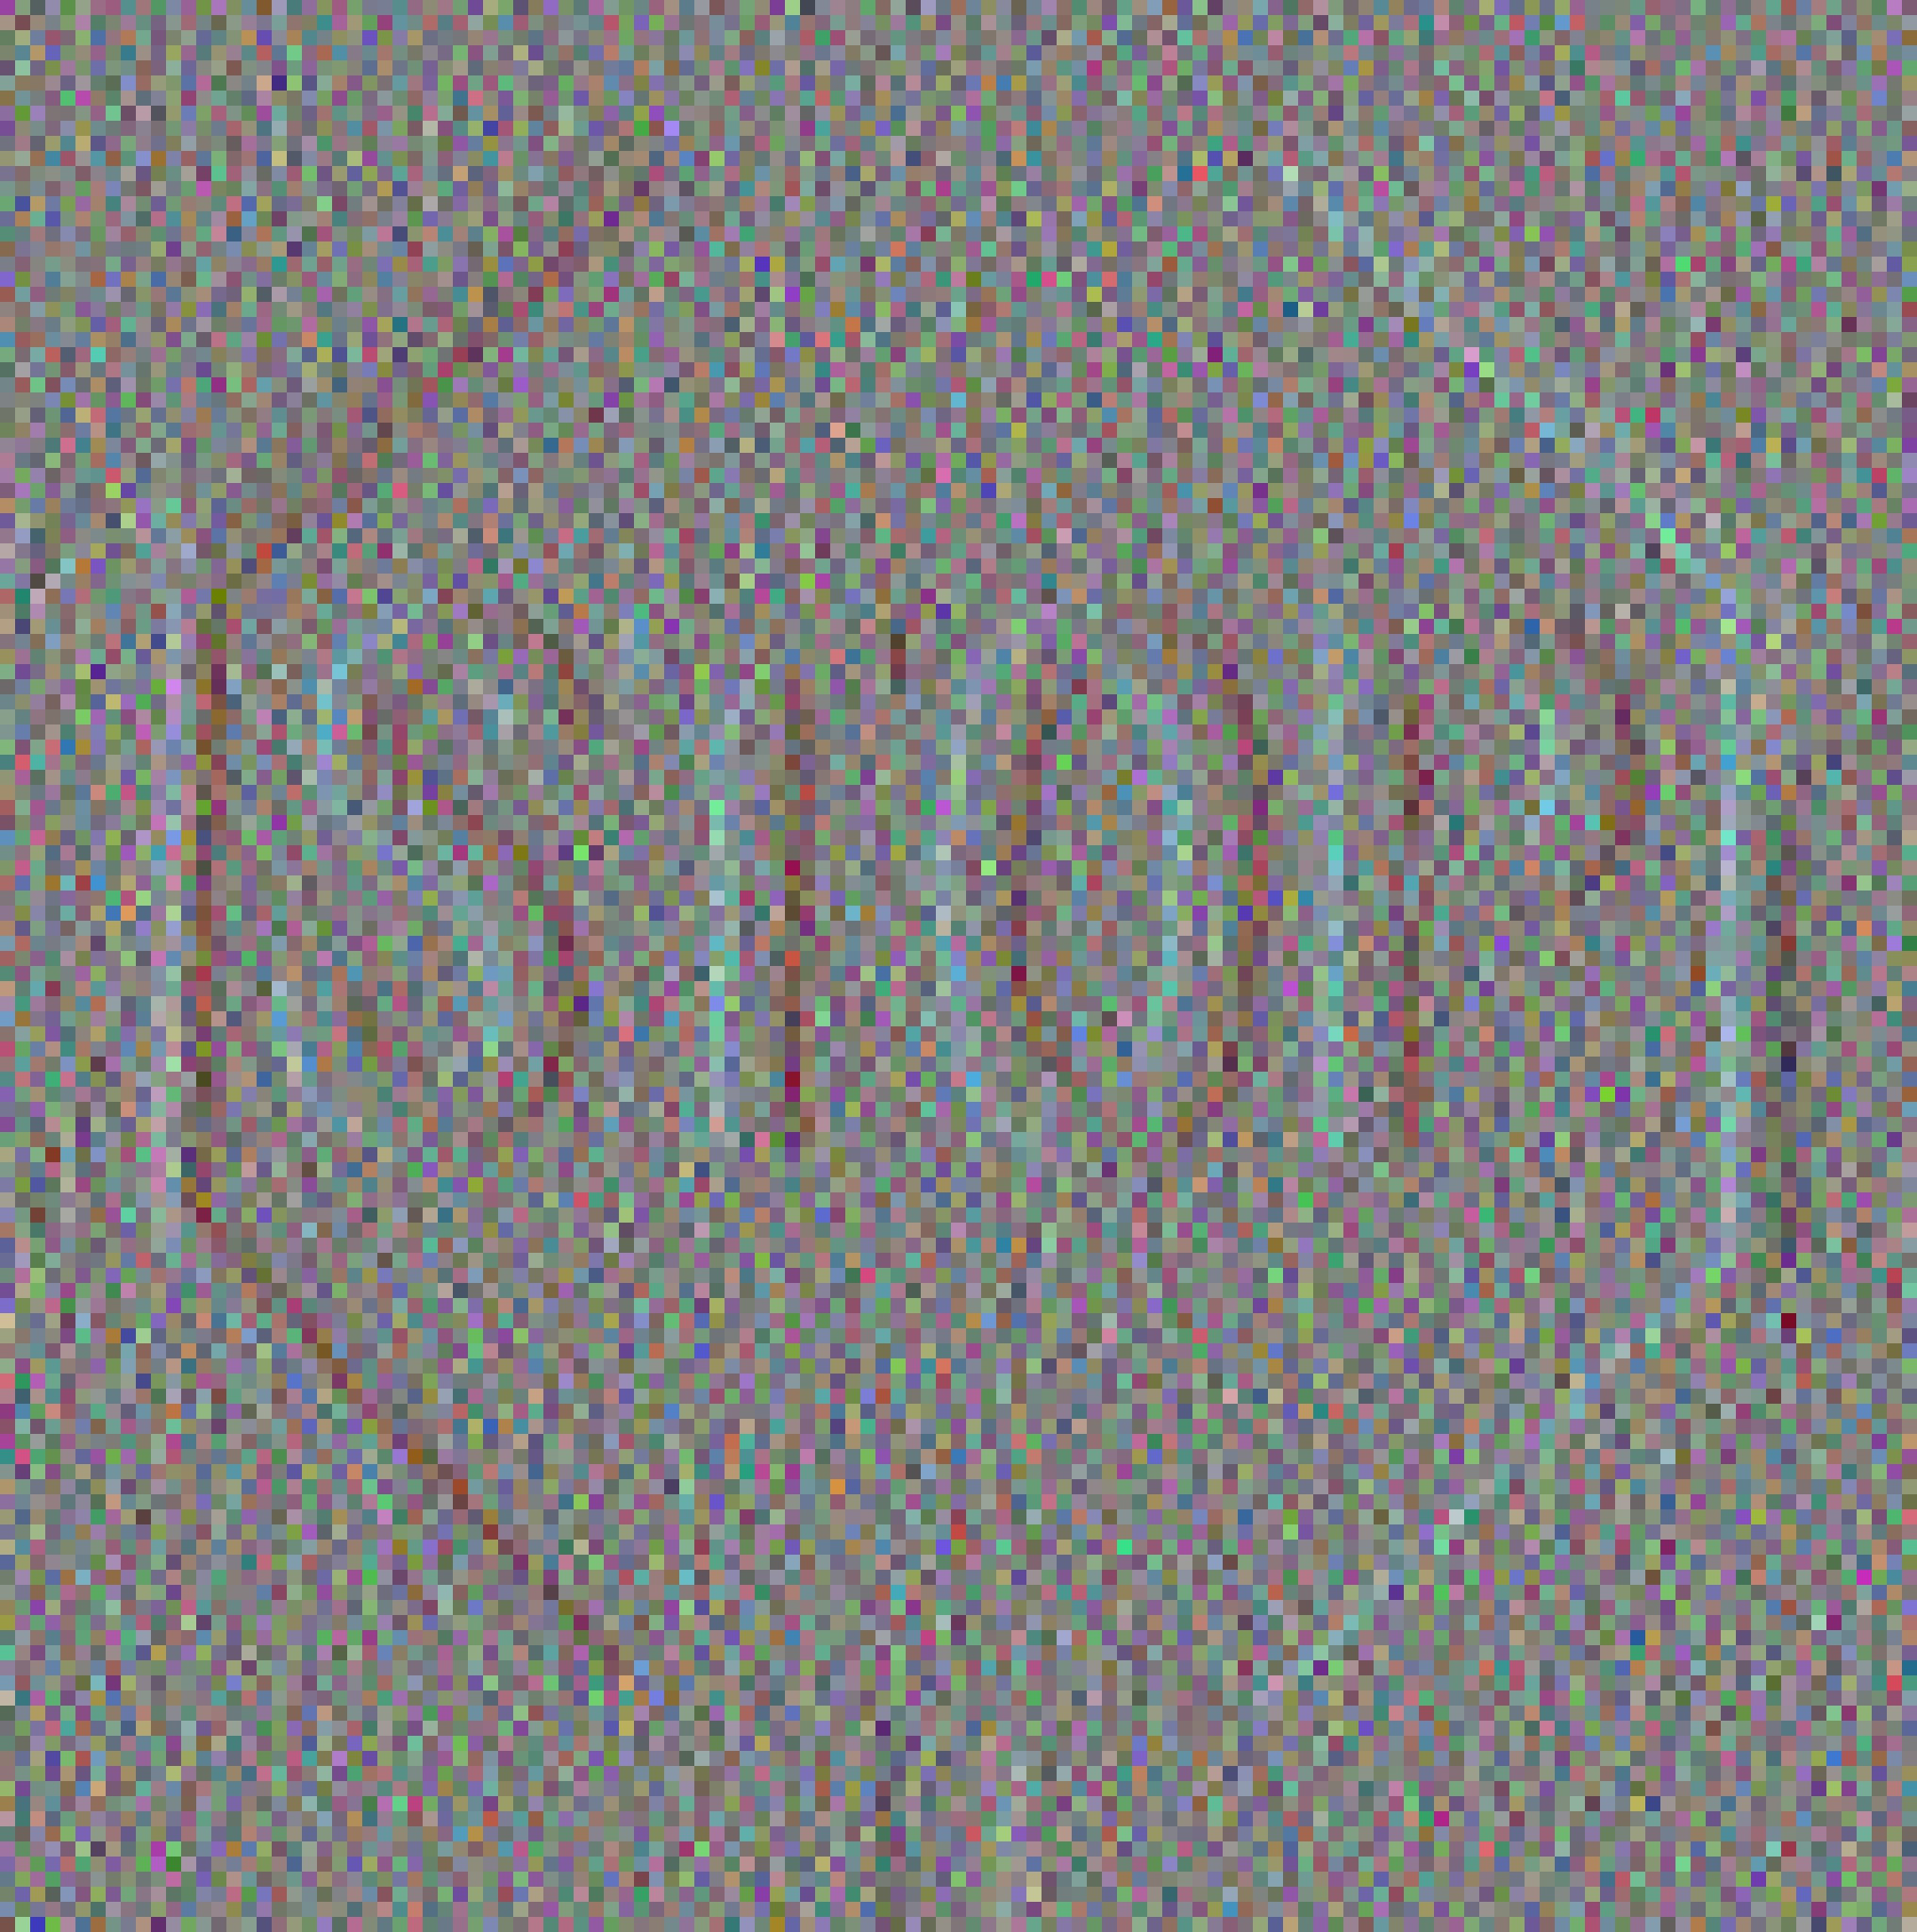
\includegraphics[width=.3\linewidth]{figures/derivatives/stop_noise_gradient.jpg}
		}
		\sublabel{c}{
			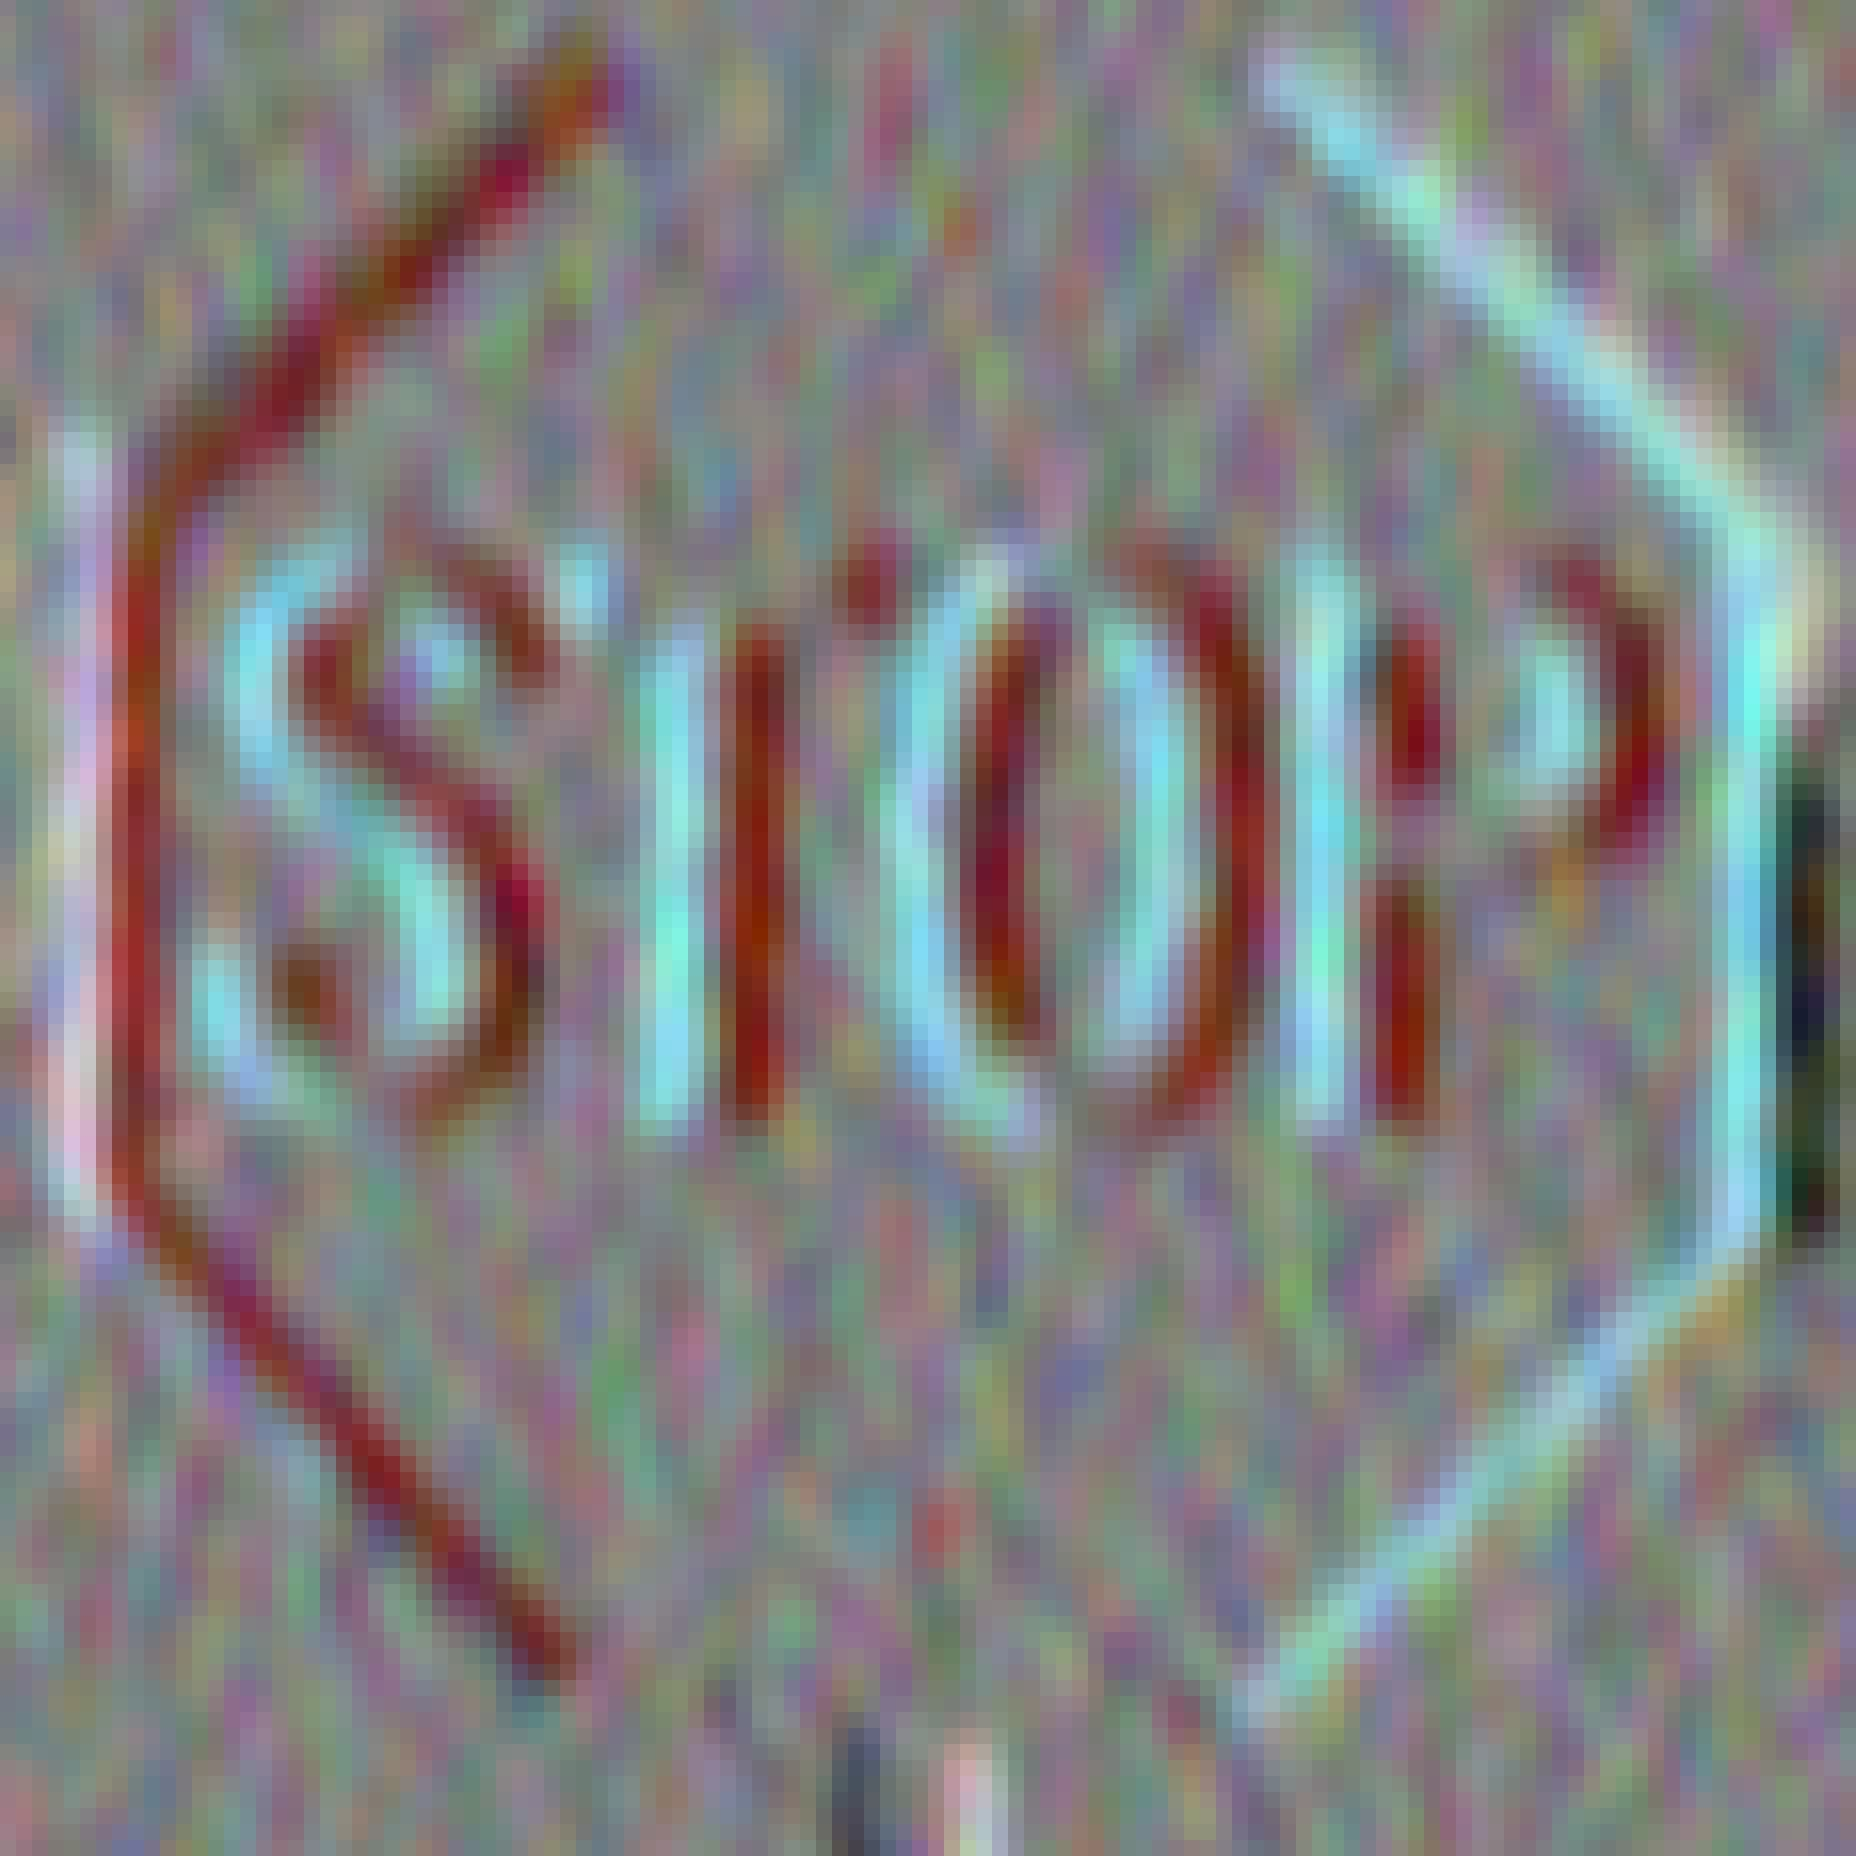
\includegraphics[width=.3\linewidth]{figures/derivatives/stop_noise_gaussian_gradient.jpg}
		}
	}
	\caption{Derivatives of a noisy image.
		(a) Input image with noise, (b) its $x$-derivative obtained by convolving with a kernel $[1, -1]$, and (c) its $x$-derivative obtained using a gaussian derivative kernel.}
	\label{fig:derivativesnoisystop}
\end{figure}

As shown in \fig{\ref{fig:derivativesnoisystop}}, the input is an image corrupted with Gaussian noise. The result of convolving the input noisy image with the kernel $[1, -1]$ results in an output with an increased noise. This is because the noise at each pixel is independent of each other, so when computing the difference between two adjacent pixels we get increased noise (the difference between two Gaussian random variables with variance $\sigma^2$ is a new Gaussian with variance $2\sigma^2$). On the other hand, the values of the  pixels of the original image are very similar and the difference is a small number (except at the object boundaries). As a consequence, the output is dominated by noise as shown in \fig{\ref{fig:derivativesnoisystop}}{b}.

There are also situations in which the derivative of an image is not defined. For instance, consider an image in the continuous domain with the form $\img (x,y) = 0$ if $x<0$ and 1 otherwise. If we try to compute $\partial \img (x,y) / \partial x$ we will get 0 everywhere, but around $x=0$ the value of the derivative is not defined. We avoided this issue in the previous section because for discrete images the approximation of the derivative is always defined.
\marginnote{Gaussian derivatives address these two issues. They where popularized by Koendering and Van Doorm \cite{Koenderink87} as a model of neurons in the visual system.}

Let's start with the following observation. For two functions defined in the continuous domain $\img(x,y)$ and $g(x,y)$, the convolution and the derivative are commutative:
\begin{equation}
	\frac {\partial \img(x,y)}{\partial x} \circ g(x,y) = \img(x,y) \circ \frac {\partial g(x,y)}{\partial x}
\end{equation}
This equality is easy to prove in the Fourier domain. If our goal is to compute image derivatives and then blur the output using a differentiable low-pass filter, $g(x,y)$, then instead of computing the derivative of the image we can compute the derivatives of the filter kernel and convolve it with the image. Even if the derivative of $\img(x,y)$ is not defined in some locations (e.g., step boundaries), we can always compute the result of this convolution.

If $g(x,y)$ is a blurring kernel it will smooth the derivatives, reducing the output noise at the expense of a loss in spatial resolution (\fig{\ref{fig:derivativesnoisystop}}[c]). A common smoothing kernel for computing derivatives is the Gaussian kernel. The Gaussian has nice smoothing properties as we discussed in the previous chapter, and it is infinitely differentiable.

If $g$ is a Gaussian, then the first order derivative is
\begin{equation}
	g_x(x,y; \sigma) = \frac {\partial g(x,y; \sigma)}{\partial x}= \frac{-x}{2 \pi \sigma^4} \exp{-\frac{x^2 +
			y^2}{2 \sigma^2}} = \frac{-x}{\sigma^2} g(x,y; \sigma)
	\label{eq:derivate1gauss2dcont}
\end{equation}

The next plots shows the 2D Gaussian with $\sigma=1$, and its $x$-derivative:
\vspace{-.2in}
\begin{figure}[h]
	\centerline{
		\sublabel{a}{
			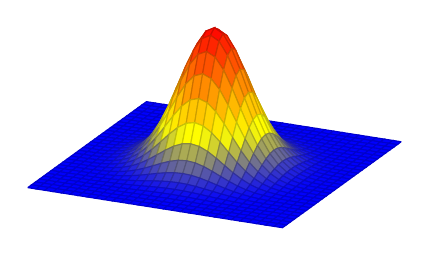
\begin{tikzpicture}
				\begin{axis}
					[width=180pt,height=150pt,
						xmin=-4, xmax=4,
						%xtick={-3, -1, 0, 1, 3},
						xlabel=$x$,
						ymin=-4, ymax=4,
						%ytick={-1,0,1},
						ylabel={$y$},
						hide axis,
						colormap/hot]
					\addplot3[domain=-4:4,samples=31,surf]
					{1/(2*pi)*exp(-(x^2+y^2)/2)};
				\end{axis}
			\end{tikzpicture}
		}
		%~&~
		%\text{(b)}
		\sublabel{b}{
			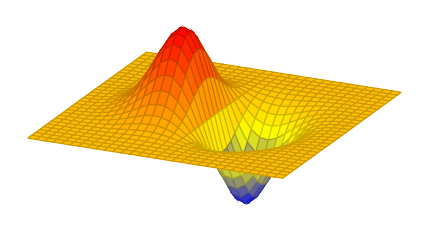
\begin{tikzpicture}
				\begin{axis}
					[width=180pt,height=150pt,
						xmin=-4, xmax=4,
						%xtick={-3, -1, 0, 1, 3},
						xlabel=$x$,
						ymin=-4, ymax=4,
						%ytick={-1,0,1},
						ylabel={$y$},
						hide axis,
						axis lines = left,
						colormap/hot]
					\addplot3[domain=-4:4,samples=31,surf]
					{1/(2*pi)*(-x)*exp(-(x^2+y^2)/2)};
				\end{axis}
			\end{tikzpicture}
		}
	}
	\caption{(a) 2D Gaussian with $\sigma=1$, and (b) its $x$-derivative.}
\end{figure}
\vspace{-.2in}


\Fig{\ref{fig:gaussiander_zebra}} shows an image filtered with three Gaussian derivatives with different widths, $\sigma$. Derivatives at different scales emphasize different aspects of the image. The fine-scale derivatives (\fig{\ref{fig:gaussiander_zebra}}[a]) highlight the bands in the zebra, while the coarse-scale derivatives (\fig{\ref{fig:gaussiander_zebra}}[c]) emphasize more the object boundaries. This multiscale image analysis will be studied in depth in the following chapter.

\begin{figure}[t]
	$
		\begin{array}{ccc}
			\text{(a)}
			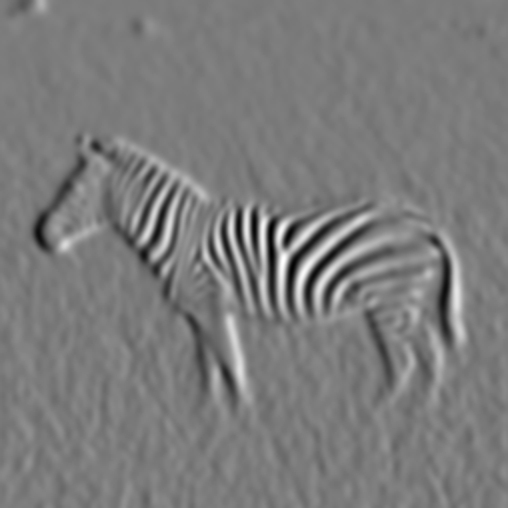
\includegraphics[width=.28\linewidth]{figures/spatial_filters/gausian_der_c_2.jpg}
			 &
			\text{(b)}
			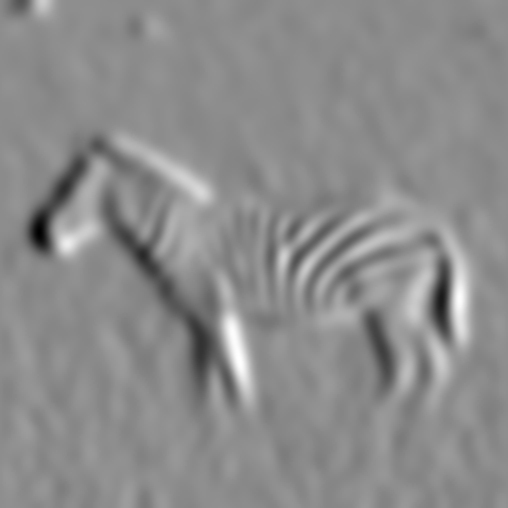
\includegraphics[width=.28\linewidth]{figures/spatial_filters/gausian_der_c_4.jpg}
			 &
			\text{(c)}
			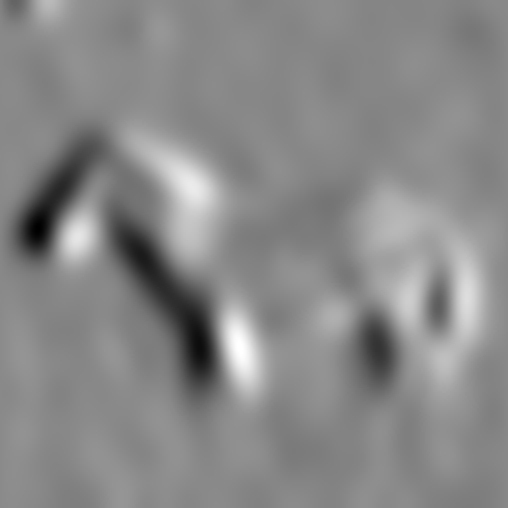
\includegraphics[width=.28\linewidth]{figures/spatial_filters/gausian_der_c_8.jpg}
			\\
			\text{(d)}
			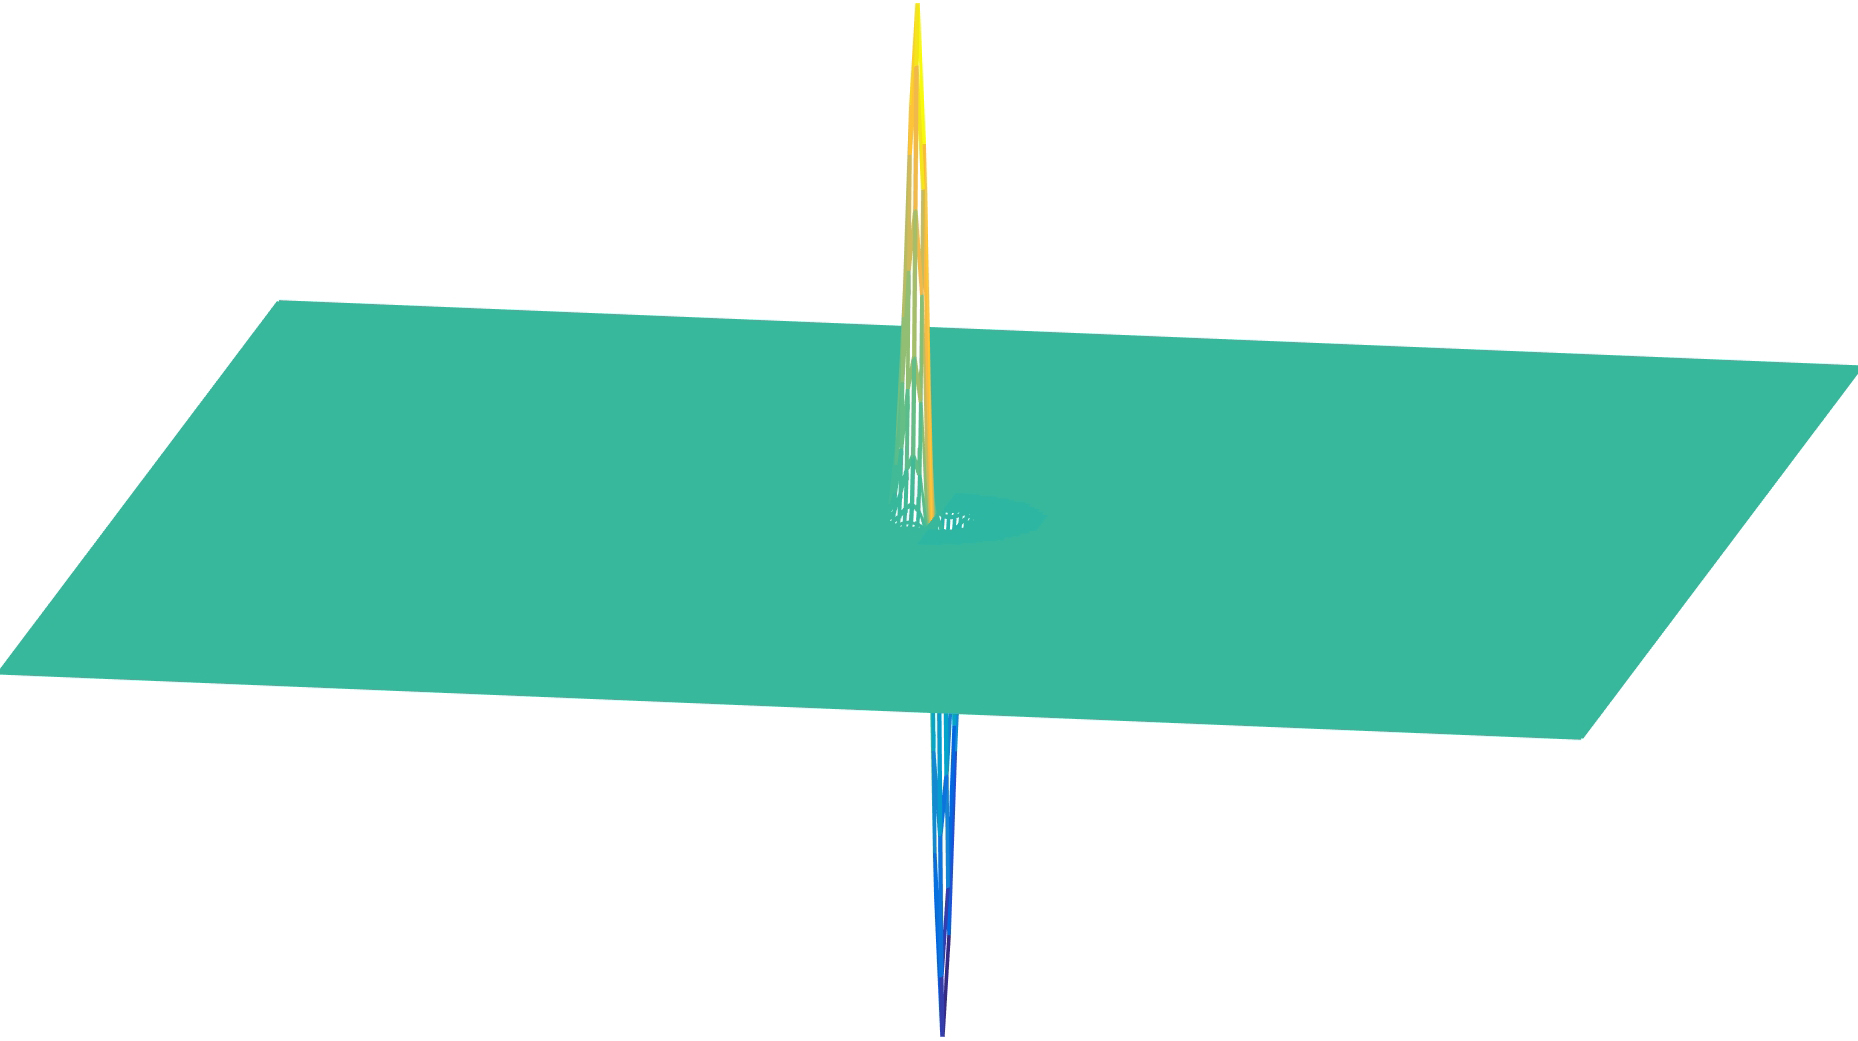
\includegraphics[width=.28\linewidth]{figures/spatial_filters/gausian_der_c_2plot.jpg}
			 &
			\text{(e)}
			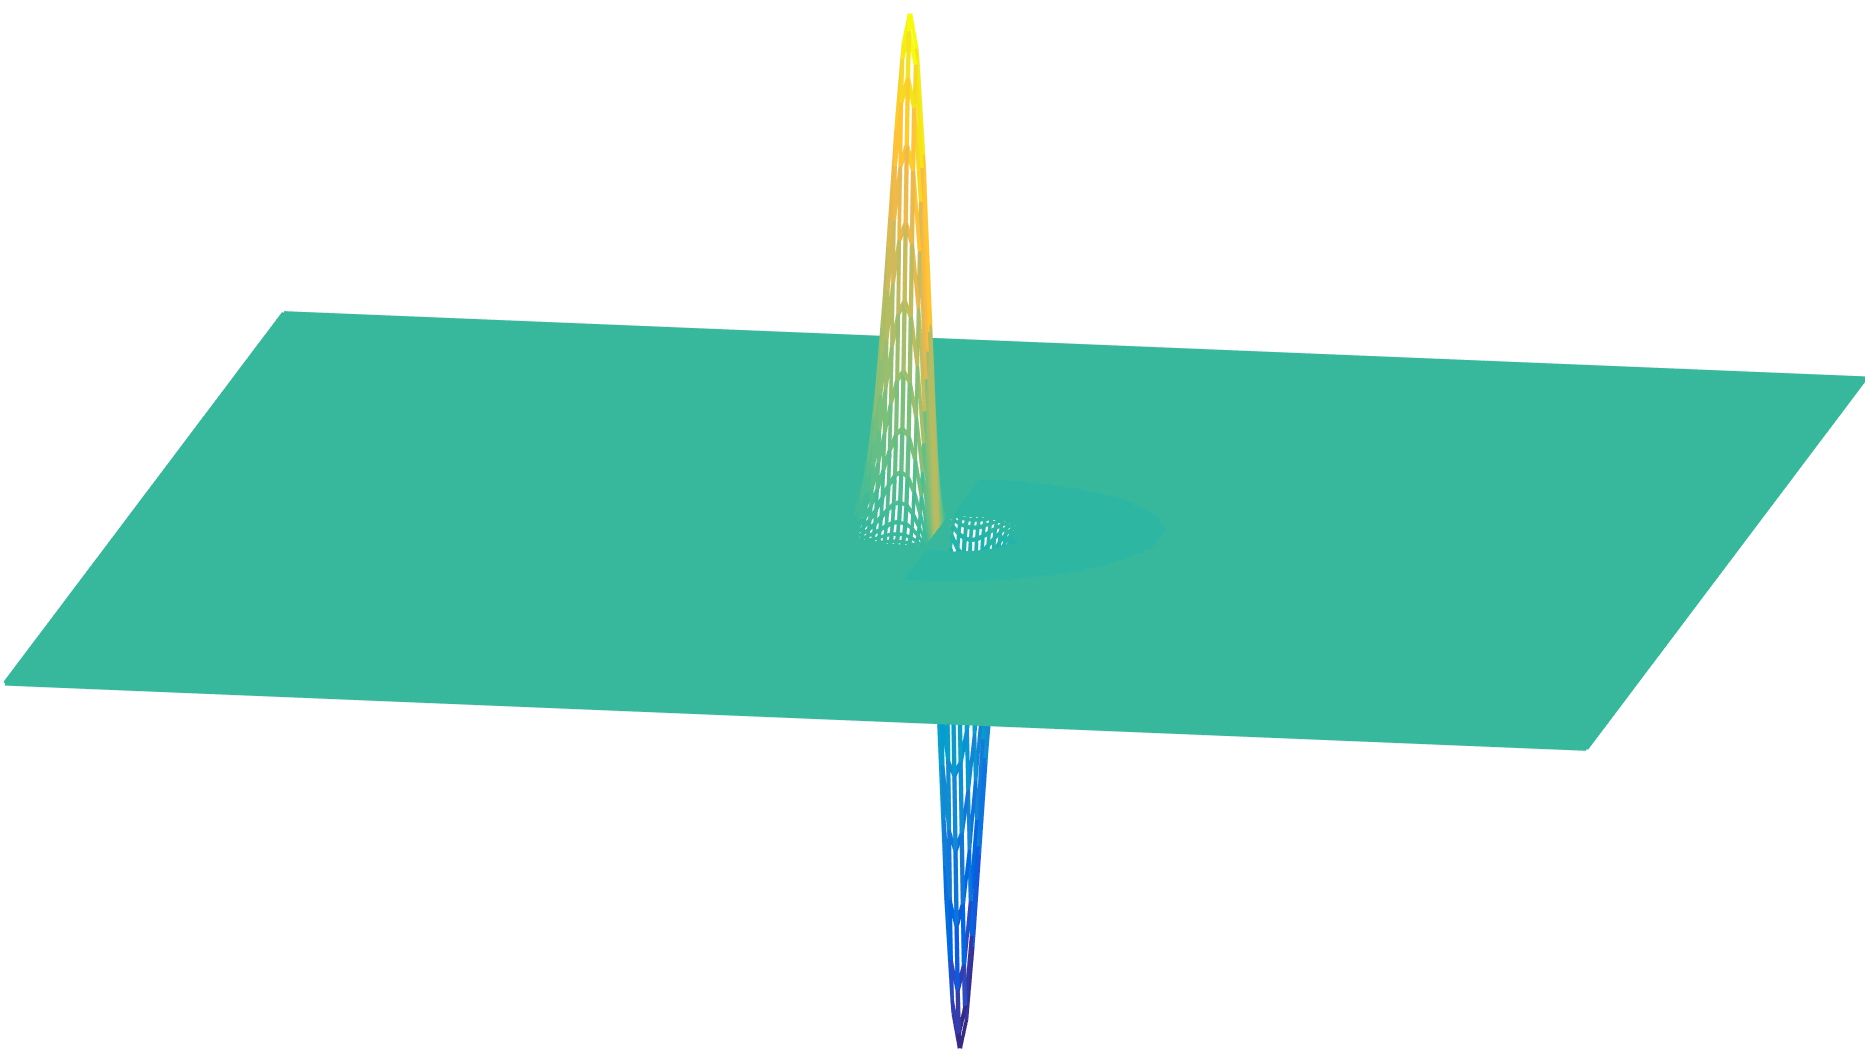
\includegraphics[width=.28\linewidth]{figures/spatial_filters/gausian_der_c_4plot.jpg}
			 &
			\text{(f)}
			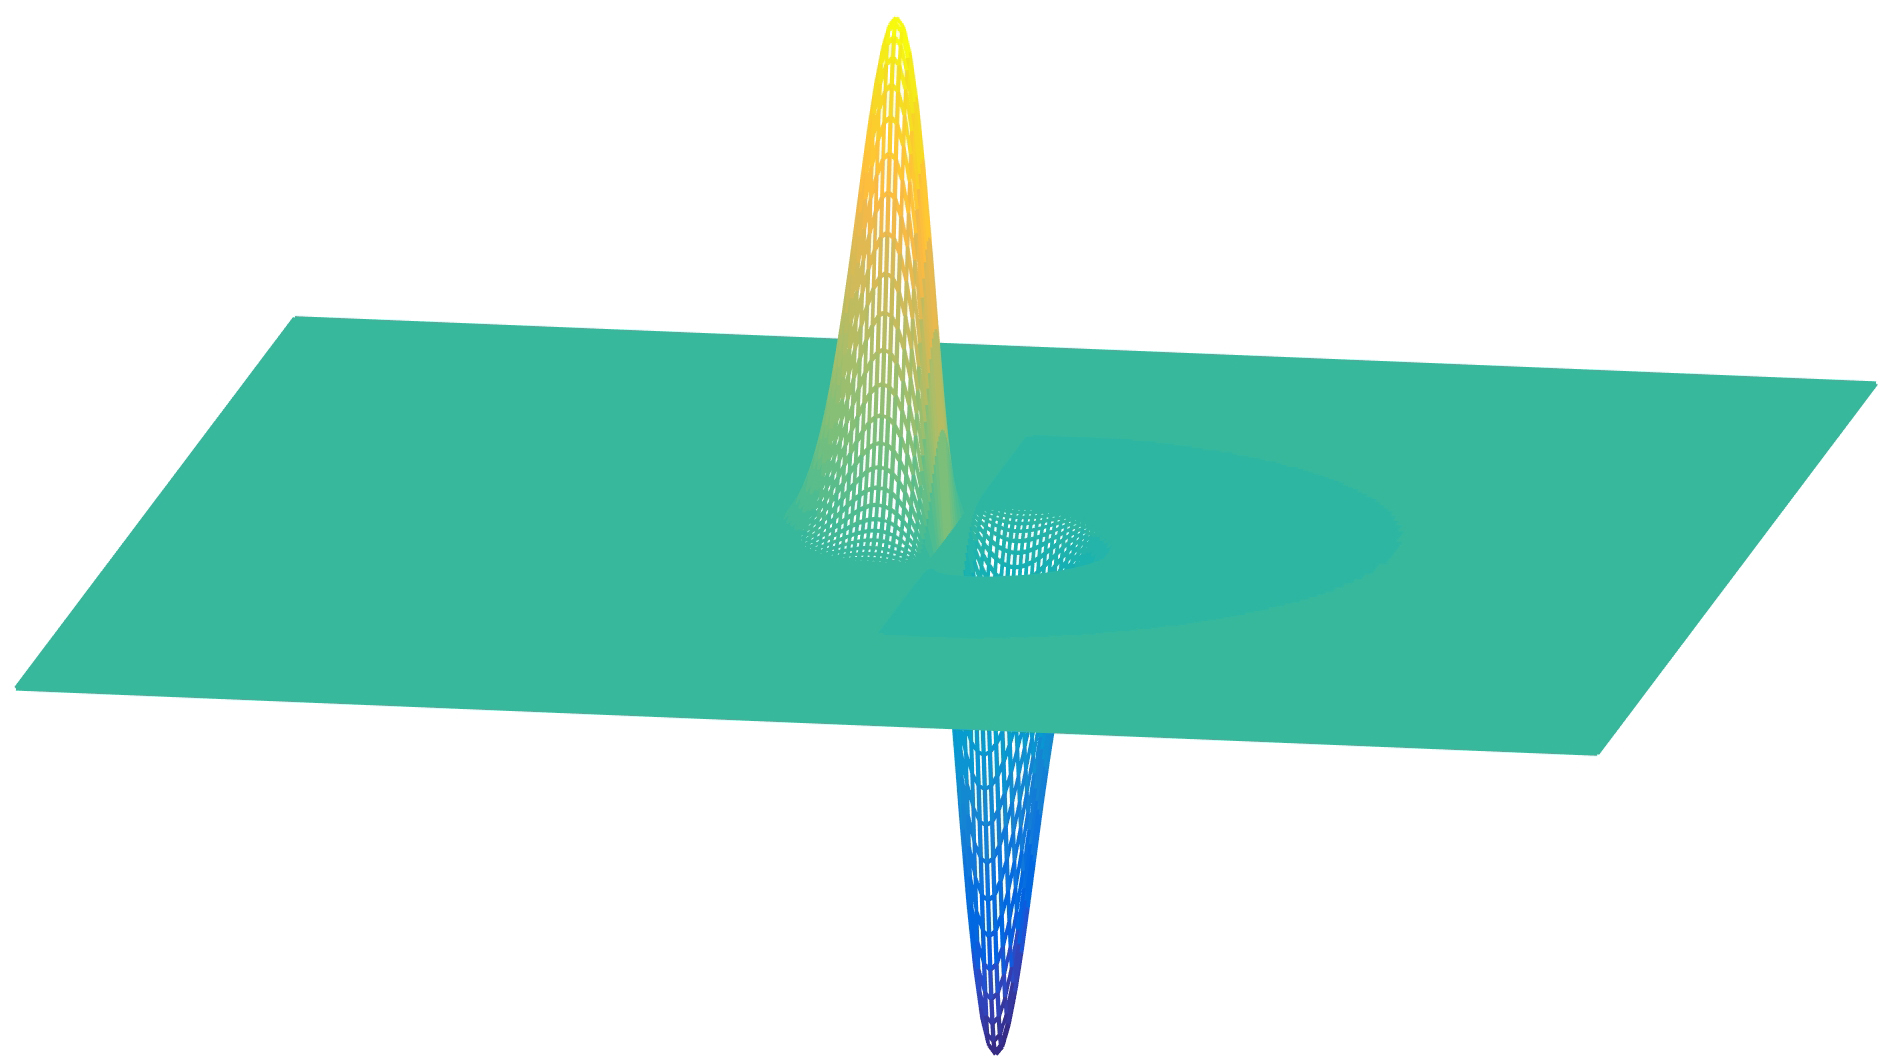
\includegraphics[width=.28\linewidth]{figures/spatial_filters/gausian_der_c_8plot.jpg}
		\end{array}
	$
	\caption{An image filtered with three Gaussian derivatives: (a) $\sigma=2$; (b) $\sigma=4$; and (c) $\sigma=8$. Plots (d-f) show the three Gaussian derivatives over the same spatial support as the image. The discrete functions are approximated by sampling the continuous Gaussian derivatives. The convolutions are performed with mirror boundary extension.}
	\label{fig:gaussiander_zebra}
\end{figure}

\section{High-Order Gaussian Derivatives}


The second order derivative of a Gaussian is
\index{Gaussian derivative!Second order derivative}
\begin{equation}
	g_{x^2}(x,y; \sigma) = \frac{x^2-\sigma^2}{\sigma^4} g(x,y; \sigma)
	\label{eq:derivate2gauss2dcont}
\end{equation}


The $n$-th order derivative of a Gaussian can be written as the product between a polynomial on $x$, with the same order as the derivative, times a Gaussian. The family of polynomials that result on computing Gaussian derivatives is called Hermite polynomials. The general expression for the $n$ derivative of a Gaussian is
\begin{equation}
	g_{x^n}(x; \sigma) =
	\frac{\partial^{n} g(x)}{\partial x^n}
	=
	\left( \frac{-1}{\sigma \sqrt{2}} \right)^n
	H_n\left( \frac{x}{\sigma \sqrt {2}} \right)
	g(x; \sigma)
	\label{eq:derivate2gauss1dhermite}
\end{equation}
The first Hermite polynomial is $H_0(x)=1$.
\index{Gaussian derivative!Hermite polynomial}
For $n=0$ we have the original Gaussian. \Fig{\ref{fig:gaussian_gaussiander}} shows the 1D Gaussian derivatives.

\begin{figure}[h!]
	\centerline{
		$
			\begin{array}{cc}
				\text{(a)}
				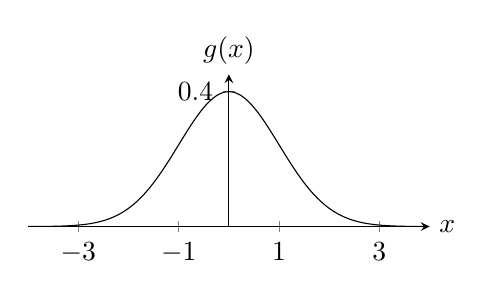
\begin{tikzpicture}
					\begin{axis} [width=190pt,height=100pt,
							axis x line=middle,
							axis y line=middle,
							tick align=center,
							every axis x label/.style={at={(current axis.right of origin)},anchor=west},
							every axis y label/.style={at={(current axis.above origin)}, anchor=north east,above=0mm},
							xmin=-4, xmax=4,
							xtick={-3, -1, 0, 1, 3},
							xlabel=$x$,
							ymin=-0, ymax=.45,
							ytick={-.1,0.4},
							ylabel={$g(x)$}]
						\addplot[domain=-4:4,samples=101,samples y=0]
						({x}, {1/(sqrt(2*pi))*exp(-x*x/2)});
					\end{axis}
				\end{tikzpicture}
				~ & ~
				\text{(b)}
				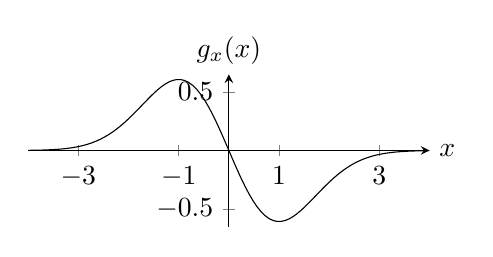
\begin{tikzpicture}
					\begin{axis} [width=190pt,height=100pt,
							axis x line=middle,
							axis y line=middle,
							tick align=center,
							every axis x label/.style={at={(current axis.right of origin)},anchor=west},
							every axis y label/.style={at={(current axis.above origin)}, anchor=north east,above=0mm},
							xmin=-4, xmax=4,
							xtick={-3, -1, 0, 1, 3},
							xlabel=$x$,
							ymin=-.65, ymax=.65,
							ytick={-0.5,0,0.5},
							ylabel={$g_x(x)$},
							color=black]
						\addplot[domain=-4:4,samples=101,samples y=0]
						({x}, {(-x)*exp(-x*x/2)});
					\end{axis}
				\end{tikzpicture}
				\\
				\text{(c)}
				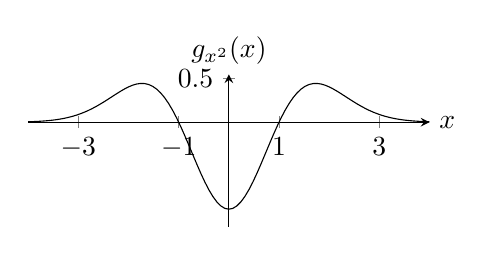
\begin{tikzpicture}
					\begin{axis} [width=190pt,height=100pt,
							axis x line=middle,
							axis y line=middle,
							tick align=center,
							every axis x label/.style={at={(current axis.right of origin)},anchor=west},
							every axis y label/.style={at={(current axis.above origin)}, anchor=north east,above=0mm},
							xmin=-4, xmax=4,
							xtick={-3, -1, 0, 1, 3},
							xlabel=$x$,
							ymin=-1.2, ymax=.55,
							ytick={0.5},
							ylabel={$g_{x^2}(x)$}]
						\addplot[domain=-4:4,samples=101,samples y=0]
						({x}, {(x*x-1)*exp(-x*x/2)});
					\end{axis}
				\end{tikzpicture}
				~ & ~
				\text{(d)}
				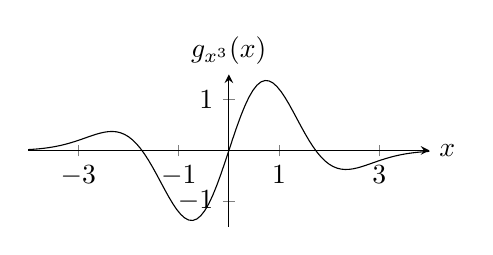
\begin{tikzpicture}
					\begin{axis} [width=190pt,height=100pt,
							axis x line=middle,
							axis y line=middle,
							tick align=center,
							every axis x label/.style={at={(current axis.right of origin)},anchor=west},
							every axis y label/.style={at={(current axis.above origin)}, anchor=north east,above=0mm},
							xmin=-4, xmax=4,
							xtick={-3, -1, 0, 1, 3},
							xlabel=$x$,
							ymin=-1.5, ymax=1.5,
							ytick={-1,0,1},
							ylabel={$g_{x^3}(x)$},
							color=black]
						\addplot[domain=-4:4,samples=101,samples y=0]
						({x}, {(-(x^3-3*x))*exp(-x*x/2)});
					\end{axis}
				\end{tikzpicture}
			\end{array}
		$
	}
	\caption{(a) 1D Gaussian with $\sigma=1$. (b–d) Gausian derivatives up to order 3.}
	\label{fig:gaussian_gaussiander}
\end{figure}


In two dimensions, as the Gaussian is separable, the partial derivatives result on the product of two Hermite polynomial, one for each spatial dimension:
\begin{equation}
	g_{x^n,y^m}(x,y; \sigma) =
	\frac{\partial^{n+m} g(x,y)}{\partial x^n \partial y^m}
	= %(-1)^{n+m}
	%\frac{1}{\sigma \sqrt{2}^{n+m}}
	\left( \frac{-1}{\sigma \sqrt{2}} \right)^{n+m}
	H_n\left( \frac{x}{\sigma \sqrt {2}} \right)
	H_m\left( \frac{y}{\sigma \sqrt {2}} \right)
	g(x,y; \sigma)
	\label{eq:derivate2gauss2dhermite}
\end{equation}
\Fig{\ref{fig:gauss_derivatives_triangle}} shows the 2D Gaussian derivatives, and \fig{\ref{fig:gauss_derivatives_triangle_FT}} shows the corresponding Fourier transforms.
\Fig{\ref{fig:gauss_derivatives_mondrian}} shows the output of the derivatives when applied to a simple input image containing a square and a circle. Different derivatives detect a diverse set of image features. However, this representation might not be very useful as it is not rotationally invariant.


\begin{figure}[t]
	\centerline{
		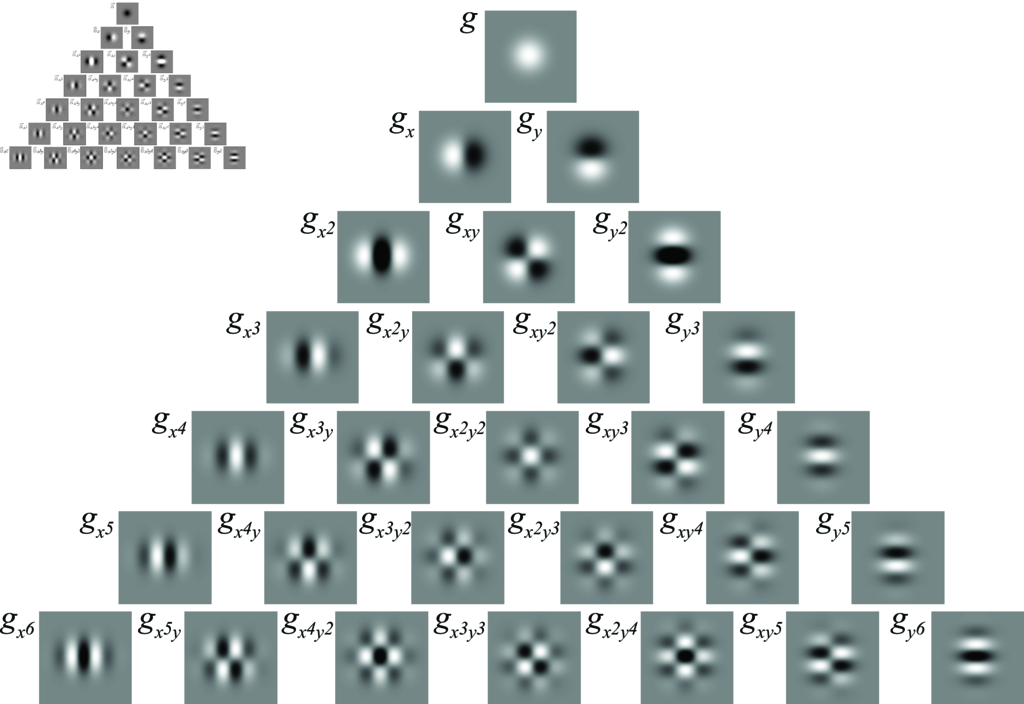
\includegraphics[width=0.8\linewidth]{figures/spatial_filters/gauss_derivatives_triangle.eps}}
	\caption{Gaussian derivatives up to order 6. All the kernels are separable. They seem similar to Fourier basis multiplied with a Gaussian window.
		\Fig{\ref{fig:gauss_derivatives_triangle_FT}} shows that they are different to sine and cosine waves, instead they look more like products of cosine and sine waves.}
	\label{fig:gauss_derivatives_triangle}
\end{figure}


\begin{figure}[t]
	\centerline{
		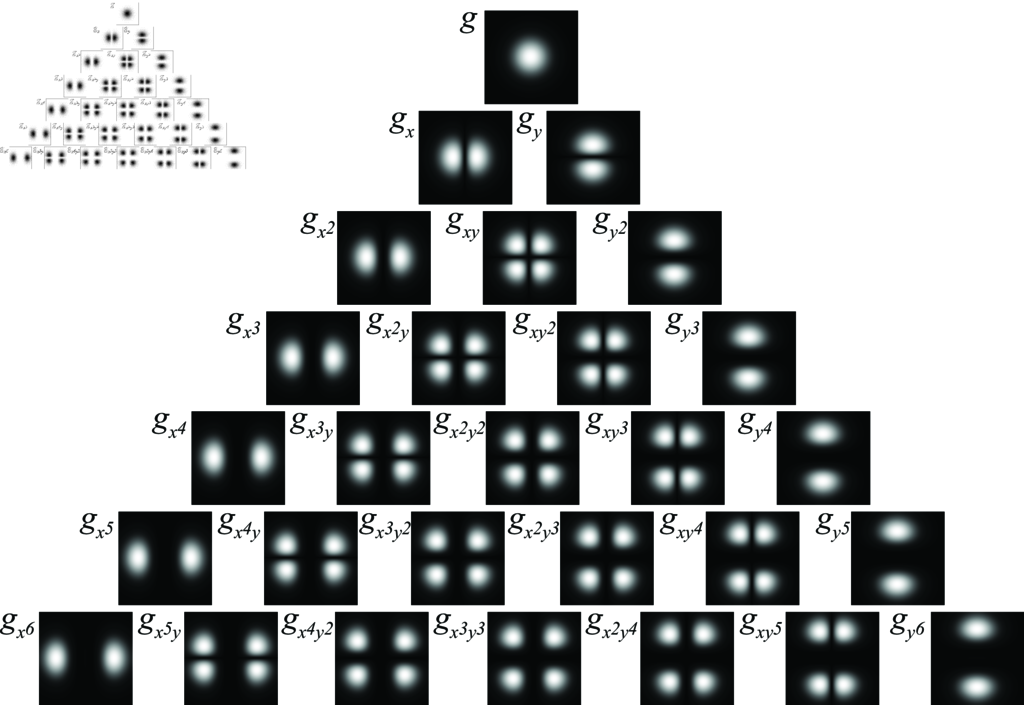
\includegraphics[width=0.8\linewidth]{figures/spatial_filters/gauss_derivatives_triangle_FT.eps}}
	\caption{Fourier transform of the Gaussian derivatives shown in \fig{\ref{fig:gauss_derivatives_triangle}}.}
	\label{fig:gauss_derivatives_triangle_FT}
\end{figure}


\begin{figure}[t]
	\centerline{
		\includegraphics[width=0.8\linewidth]{figures/derivatives/fig_gauss_derivatives_triangle_mondrian.eps}}
	\caption{An image containing a square and a circle and its output to the Gaussian derivatives up to order 3.}
	\label{fig:gauss_derivatives_mondrian}
\end{figure}


The Gaussian derivatives share many of the properties of the Gaussian. The convolution of two Gaussian derivatives of order $n$ and $m$ and variances $\sigma_1^2$ and $\sigma_2^2$ result in another Gaussian derivative of order $n+m$ and variance $\sigma_1^2 + \sigma_2^2$. Proving this property on the spatial domain can be tedious. However, it is trivial to prove it in the Fourier domain.







\section{Derivatives of Binomial Filters}
\label{sec:derivatives_binomial_filters}
When processing images we have to use discrete approximations for the Gaussian derivatives. After discretization, many of the properties of the continuous Gaussian will not hold exactly.

There are many discrete approximations. For instance, we can take samples of the continuous functions. In practice it is common to use the discrete approximation given by the binomial filters. \Fig{\ref{fig:derivativepascaltriangle}} shows the result of convolving the binomial coefficients, $b_n$, with  $\left[1, -1\right]$.

\begin{figure}[h!]
	\centerline{
		%\[
		$\begin{array}{ccccccccccccccccccccl}
				d_0 & ~ & ~ & ~ & ~    & ~    & ~    & ~    & ~    & ~~1  & ~~~ & -1  & ~  & ~  & ~  & ~  & ~  & ~ & ~ & ~ & \\
				d_1 & ~ & ~ & ~ & ~    & ~    & ~    & ~    & ~~1  & ~    & ~~0 & ~   & -1 & ~  & ~  & ~  & ~  & ~ & ~ & ~ & \\
				d_2 & ~ & ~ & ~ & ~    & ~    & ~    & ~~~1 & ~    & ~~~1 & ~~~ & -1  & ~  & -1 & ~  & ~  & ~  & ~ & ~ & ~ & \\
				d_3 & ~ & ~ & ~ & ~    & ~    & ~~~1 & ~    & ~~~2 & ~    & ~~0 & ~~~ & -2 & ~  & -1 & ~  & ~  & ~ & ~ & ~ & \\
				d_4 & ~ & ~ & ~ & ~    & ~~~1 & ~    & ~~~3 & ~    & ~~~2 & ~~~ & -2  & ~  & -3 & ~  & -1 & ~  & ~ & ~ & ~ & \\
				d_5 & ~ & ~ & ~ & ~~~1 & ~    & ~~~4 & ~    & ~~~5 & ~    & ~~0 & ~   & -5 & ~  & -4 & ~  & -1 & ~ & ~ & ~ &
			\end{array}$
		%\]
	}
	\caption{Derivative of binomial coefficients resulting from the convolution $b_n \circ \left[1, -1\right]$. The filters, $d_0$ and $d_1$, are the ones we have studied in the previous section.}
	\label{fig:derivativepascaltriangle}
\end{figure}

In two dimensions, we can use separable filters and build a partial derivative as
\begin{equation}
	Sobel_x =  \begin{bmatrix}
		1 ~ & 0 ~ & -1 \\
	\end{bmatrix}\circ \begin{bmatrix}
		1 \\
		2 \\
		1
	\end{bmatrix}=
	\begin{bmatrix}
		1 ~ & 0 ~ & -1 \\
		2 ~ & 0 ~ & -2 \\
		1~  & 0 ~ & -1
	\end{bmatrix}
\end{equation}
\begin{equation}
	Sobel_y =  \begin{bmatrix}
		-1 & -2 & -1 \\
		~0 & ~0 & ~0 \\
		~1 & ~2 & ~1
	\end{bmatrix}
	\label{eq:sobel_kernels}
\end{equation}
This particular filter is called the {\bf Sobel-Feldman operator}.
\index{Sobel-Feldman operator}
The goal of this operator was to be compact and to be as isotropic as possible. The Sobel-Feldman operator can be implemented very efficiently as it can be written as the convolution with four small kernels, $Sobel_x=b_1 \circ d_0 \circ b_1^T \circ b_1^T$.
\marginnote{Remember that $b_1=[1, 1]$, and $b_2=b_1 \circ b_1 = [1,2,1]$.}
The DFT of the Sobel-Feldman operator is
\begin{equation}
	Sobel_x \left[u,v \right] = D_1\left[u\right] B_2 \left[v \right] = j \sin \left( 2 \pi u /N \right) \left( 2+2 \cos \left(2 \pi v/N \right) \right)
\end{equation}
and it is shown in \fig{\ref{fig:DFTderivativeoperators}}{d}. $N \times N$ is the extension of the domain (the operator is zero padded). As $d_0$ and $d_1$ are 1D their 2D DFT vary only along one dimension. The Roberts cross operator is similar to a rotated version of $d_1$. The Sobel-Feldman operator has the profile of $D_1$ along the axis $u=0$ and it is proportional to the profile of $B_2$ along any section $v=constant$.
\index{Roberts cross operator}

\begin{figure}[t]
	\centerline{
		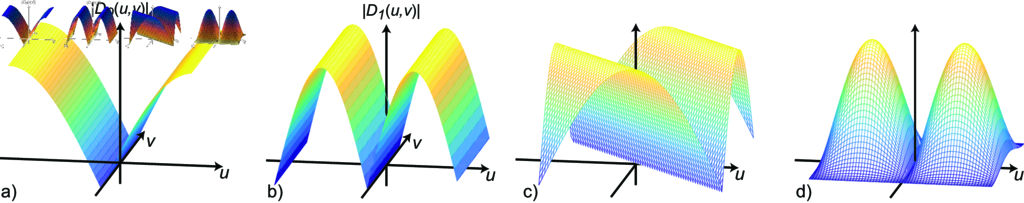
\includegraphics[width=1\linewidth]{figures/spatial_filters/DFTderivativeoperators.eps}}
	\caption{Magnitude of the DFT of four different discretization of Gaussian derivatives: (a) $d_0$; (b) $d_1$; (c) Robert cross operator; and (d) Sobel-Feldman operator.
	}
	\label{fig:DFTderivativeoperators}
\end{figure}

\Fig{\ref{fig:DFTderivativeoperators}} compares the DFT of the four types of approximations of the derivatives that we have discussed. These operators are still very popular. $Sobel$ has the best tolerance to noise due to its band-pass nature. The kernel $d_0$ is the one that provides the highest resolution in the output. \Fig{\ref{fig:circle}} shows the output of different derivative approximations to a simple input image containing a circle. In the next section we will discuss how to use these derivatives to extract other interesting quantities.

% Sobel, I., Feldman, G., "A 3x3 Isotropic Gradient Operator for Image Processing", presented at the Stanford Artificial Intelligence Project (SAIL) in 1968. never published as a paper.
% https://www.researchgate.net/publication/239398674_An_Isotropic_3_3_Image_Gradient_Operator

\begin{figure}[t]
	\centerline{
		\includegraphics[width=1\linewidth]{figures/spatial_filters/circle.eps}}
	\caption{Derivatives of a circle along the directions $n$, $m$, and 45 degrees.
		%And also the magnitude and the angle of the gradient. 
		The angle is shown only where the magnitude is $>0$. The derivative output along 45 degrees is obtained as a linear combination of the derivatives outputs along $n$ and $m$. Check the differences among the different kernels. The Sobel operator gives the most rotationally invariant gradient magnitude, but it is blurrier.
		%at the expense of a bit of blurring of the output.
	}
	\label{fig:circle}
\end{figure}

\section{Image Gradient and Directional Derivatives}

As we saw in \chap{\ref{chapter:simplesystem}}, an important image representation is given by the image gradient. From the image derivatives we can define also the image gradient as the vector:
\begin{equation}
	\nabla \img (x,y) = \left( \frac{\partial \img(x,y)}{\partial x}, \frac{\partial \img(x,y)}{\partial y} \right)
\end{equation}
For each pixel, the output is a 2D vector.  In the case of using Gaussian derivatives, we can write:
\begin{equation}
	\nabla \img \circ g = \nabla g \circ \img = \left( g_x(x,y), g_y(x,y) \right) \circ \img
\end{equation}

Although we have mostly computed derivatives along the $x$ and $y$ variables, we can obtain the derivative on any orientation as a linear combination of the two derivatives along the main axes. With ${\bf t}=\left( \cos (\theta), \sin(\theta) \right)$, we can write the directional derivative a long the vector ${\bf t}$ as:
\begin{equation}
	\frac{\partial \img (x,y)}{\partial {\bf t}} =  \nabla \img \cdot {\bf t} = \cos(\theta) \frac{\partial \img}{\partial x} + \sin(\theta) \frac{\partial \img}{\partial y}
\end{equation}
In the Gaussian case:
\begin{equation}
	\frac{\partial \img}{\partial {\bf t}} \circ g = \left( \cos(\theta) g_x(x,y) + \sin(\theta) g_y(x,y) \right) \circ \img = \left( \nabla g  \cdot {\bf t} \right) \circ \img
	= g_{\theta} (x,y)  \circ \img
	\label{eq:steerable_derivative_filter}
\end{equation}
with $g_{\theta} (x,y) = \cos(\theta) g_x(x,y) + \sin(\theta) g_y(x,y)$. However, to compute the derivative along any arbitrary angle $\theta$ does not require doing new convolutions. Instead, we can compute any derivative as a linear combination of the output of convolving the image with $g_x(x,y)$ and $g_y(x,y)$:
\begin{equation}
	\frac{\partial \img}{\partial {\bf t}} \circ g =  \cos(\theta) g_x(x,y) \circ \img + \sin(\theta) g_y(x,y) \circ \img
\end{equation}

When using discrete convolutional kernels $d_n\left[n,m\right]$ and $d_m\left[n,m\right]$ to approximate the derivatives along $n$ and $m$, it can be written as
\begin{equation}
	\nabla \img = \left( d_n\left[n,m\right], d_m\left[n,m\right] \right) \circ \img \left[n,m\right]
\end{equation}
and
\begin{equation}
	\nabla \img \cdot {\bf t} =d_{\theta} \left[n,m\right] \circ \img \left[n,m\right]
\end{equation}
with $d_{\theta} \left[n,m\right]  = \cos(\theta) d_n\left[n,m\right] + \sin(\theta) d_m\left[n,m\right]$. We expect that the linear combination of these two kernels should approximate the derivative along the direction $\theta$. The quality of this approximation will vary for the different kernels we have seen in the previous sections.





%- The structure tensor: this is an example of a powerful image derivative representation. And we will see more of it (or related) later.

% - link to the work on scale space

\section{Image Laplacian}

The {\bf Laplacian filter}
\index{Filter!Laplacian}
was made popular by Marr and Hildreth in 1980 \cite{Marr80} in the search for operators that locate the boundaries between objects. The Laplacian is a common operator from differential geometry to measure the divergence of the gradient and it appears frequently in modeling fields in physics.
The Laplacian also has applications in graph theory and in spectral methods for image segmentation \cite{ng2002}.
%Can one hear the shape of a drum. The American Mathematical Monthly, vol. 73, 1966, Part II, pp. 1-23

\marginnote{One example of application of the Laplacian is in the paper \booktitle{Can One Hear the Shape of a Drum} \cite{Kac_1966} where the Laplacian is used for modeling vibrations in a drum and the sounds it produces as a function of its shape.}[-.5in]

The  Laplacian operator is defined as the sum of the second order partial derivatives of a function:
% Marr, D.; Hildreth, E. (29 Feb 1980), "Theory of Edge Detection", Proceedings of the Royal Society of London. Series B, Biological Sciences 207 (1167): 187�217

\begin{equation}
	\nabla^2 \img = \frac{\partial^2 \img}{\partial x^2} + \frac{\partial^2 \img}{\partial y^2}
\end{equation}

The Laplacian is more sensitive to noise than the first order derivative. Therefore, in the presence of noise,  when computing the Laplacian operator on an image $\img(x,y)$, it is useful to smooth the output with a Gaussian kernel, $g(x,y)$. We can write,
\begin{equation}
	\nabla^2 \img \circ g = \nabla^2 g \circ \img
\end{equation}
Therefore, the same result can be obtained if we first compute the Laplacian of the Gaussian kernel, $g(x,y)$ and then convolve it with the input image. The Laplacian of the Gaussian is
\begin{equation}
	\nabla^2 g = \frac{x^2 + y^2 -2\sigma^2}{\sigma^4} g(x,y)
\end{equation}

The next plot (\fig{\ref{fig:mexican_hat_wavelet}}) shows the Gaussian Laplacian ($sigma = 1$). Due to its shape, the Laplacian is also called the inverted {\bf mexican hat wavelet}. Despite that visually it might seem as if the Laplacian has a negative mean value, the mean is actually zero as the positive side is wider than the negative.
\index{Mexican hat wavelet}

\begin{figure}[h]
	\centerline{
		\sublabel{a}{
			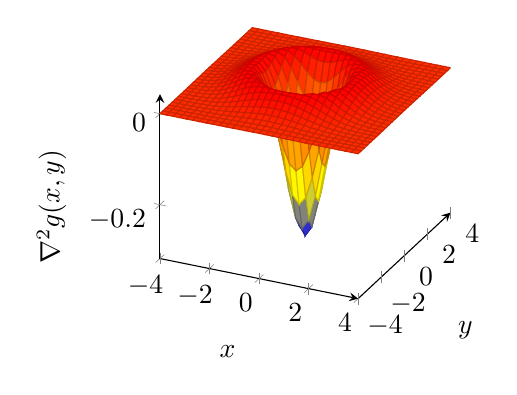
\begin{tikzpicture}
				\begin{axis}
					[width=150pt,height=150pt,
						xmin=-4, xmax=4,
						%xtick={-3, -1, 0, 1, 3},
						xlabel=$x$,
						ymin=-4, ymax=4,
						%ytick={-1,0,1},
						ylabel={$y$},
						%hide axis,
						zlabel={$\nabla^2 g(x,y)$},
						axis lines = left,
						colormap/hot]
					\addplot3[domain=-4:4,samples=31,
						surf]
					{1/(2*pi)*(x^2+y^2-2)*exp(-(x^2+y^2)/2)};
				\end{axis}
			\end{tikzpicture}
		}
		\sublabel{b}{
			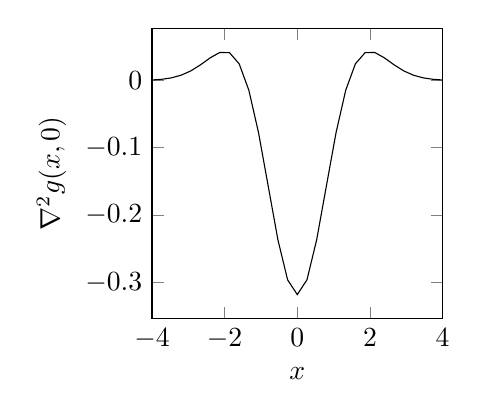
\begin{tikzpicture}
				\begin{axis}
					[width=150pt,height=150pt,
						xmin=-4, xmax=4,
						%xtick={-3, -1, 0, 1, 3},
						xlabel=$x$,
						%ymin=-4, ymax=4,
						%ytick={-1,0,1},
						ylabel={$\nabla^2 g(x,0)$},
						%hide axis,
						%axis lines = left,
						%colormap/hot
					]
					\addplot[domain=-4:4,samples=31]
					{1/(2*pi)*(x^2-2)*exp(-(x^2)/2)};
				\end{axis}
			\end{tikzpicture}
		}
	}
	\caption{The Gaussian Laplacian ($sigma = 1$) is also called the inverted {\bf mexican hat wavelet}. (a) 2D plot. (b) 1D section at $y=0$.}
	\label{fig:mexican_hat_wavelet}
\end{figure}



In the discrete domain there are several approximations to the Laplacian filter. The simplest one consists in sampling the continuous Gaussian Laplacian in discrete locations.
Figures {\ref{fig:DFTlaplacians}}(a-c) shows the DFT of the Gaussian Laplacian for three different values of $\sigma$. For values $\sigma>1$ the resulting filter is band-pass, which is the expected behavior for the Gaussian Laplacian. %\fig{\ref{fig:DFTlaplacians}}{d} shows the DFT of the five-point discrete approximation to the laplacian.

\begin{figure}[h!]
	\centerline{
		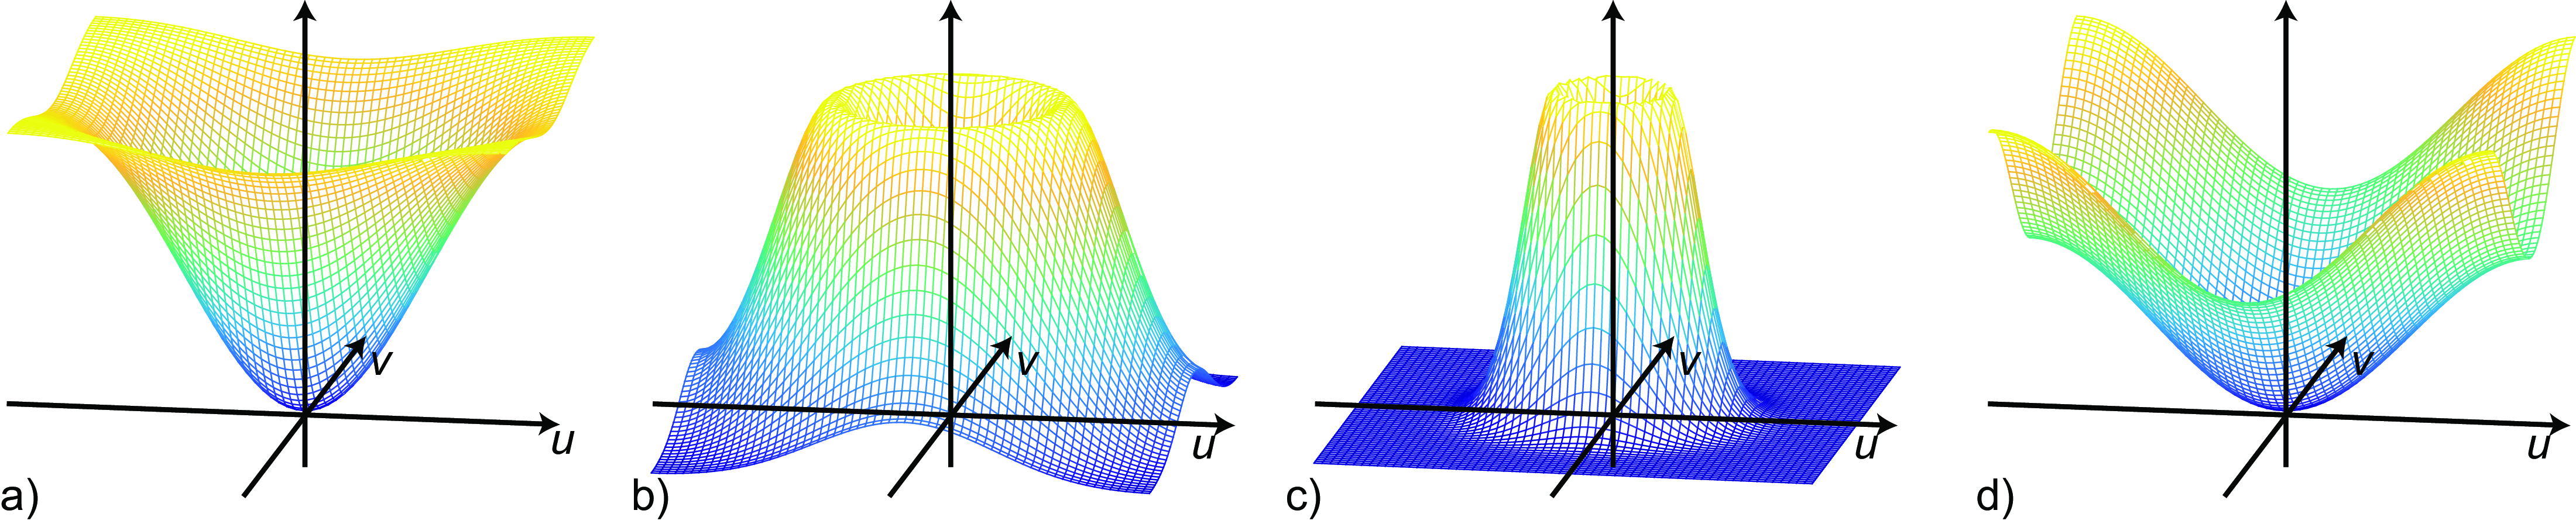
\includegraphics[width=1\linewidth]{figures/spatial_filters/DFTlaplacians.eps}}
	\caption{Magnitude of the DFT of the Gaussian Laplacian with (a) $\sigma=1/2$; (b) $\sigma=1$; (c) $\sigma=2$; and (d) DFT of the five-point discrete approximation, \eqn{\ref{eq:five_point_laplacian}}.
	}
	\label{fig:DFTlaplacians}
\end{figure}

%Lindeberg \cite{} explored different approximations to the image Laplacian in order to optimize its properties. 

In one dimension, the Laplacian can be approximated by $\left[ 1,-2,1 \right]$, which is the result of the convolution of two 2-tap discrete approximations of the derivative $\left[1,-1 \right] \circ \left[1,-1 \right]$.
% ftp://ftp.nada.kth.se/CVAP/reports/cvap66.pdf
In two dimensions, the most popular approximation is the five-point formula, which consists in convolving the image with the kernel:
\begin{equation}
	\nabla_5^2 =
	\begin{bmatrix}
		0 & 1  & 0 \\
		1 & -4 & 1 \\
		0 & 1  & 0
	\end{bmatrix}
	\label{eq:five_point_laplacian}
\end{equation}
It involves the central pixel and its four nearest neighbors. This is a sum-separable kernel: it corresponds to approximating the second-order derivative for each coordinate and summing the result (i.e., convolve the image with $\left[1,-2,1\right]$ and also with its transpose and summing the two outputs).
%It is important to shift by one pixel, on the appropriate dimension, the two results to make sure that the sum results in the Laplacian.) 
\Fig{\ref{fig:DFTlaplacians}}{d} shows the DFT of this approximation. It also has a quadratic from near the origin of the frequency domain, but it has a high-pass shape similar to the one obtained for a small value of $\sigma$.

\marginnote{
	The Laplacian of the image, using the five-point formula, is:
	\begin{equation*}
		\nabla_5^2 \img[n,m] = -4 \img[n,m]
		+ \img[n+1,m]
		+ \img[n-1,m]
		+ \img[n,m+1]
		+ \img[n,m-1]
	\end{equation*}
}


\Fig{\ref{fig:wheellaplacian}} compares the output of image derivatives and the Laplacian. Note that when summing two first-order derivatives along $x$ and $y$, what we obtain is a first-order derivative along the 45 degree angle. However, when summing up the two second-order derivatives we obtain a rotationally invariant kernel, as shown in \fig{\ref{fig:wheellaplacian}}{d}.


\begin{figure}[h]
	\centerline{
		\sublabel{a}{
			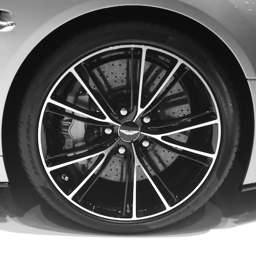
\includegraphics[width=.2\linewidth]{figures/spatial_filters/wheel256.jpg}}
		\sublabel{b}{
			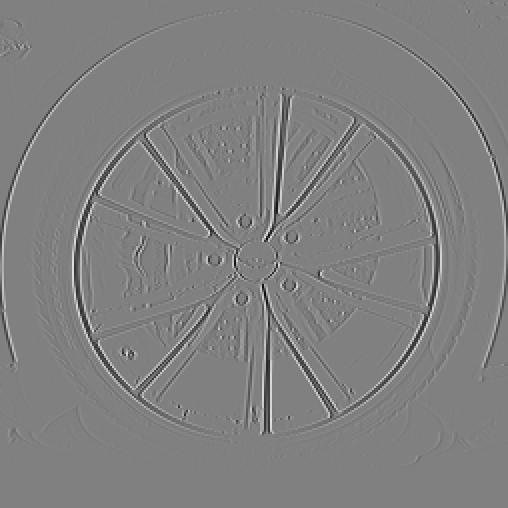
\includegraphics[width=.2\linewidth]{figures/spatial_filters/wheelLaplacianx.jpg}}
		\sublabel{c}{
			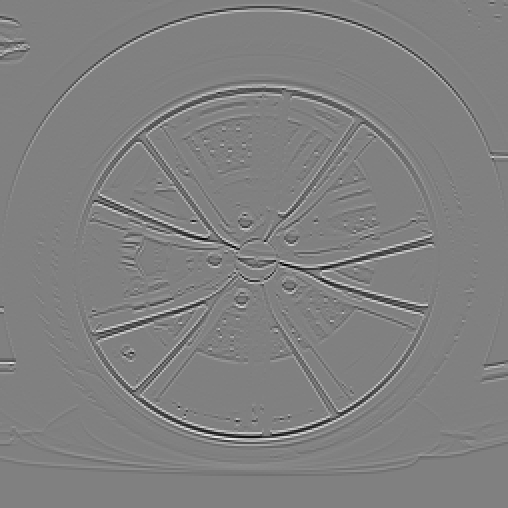
\includegraphics[width=.2\linewidth]{figures/spatial_filters/wheelLaplaciany.jpg}}
		\sublabel{d}{
			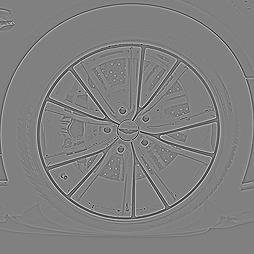
\includegraphics[width=.2\linewidth]{figures/spatial_filters/wheelLaplacian.jpg}}
	}
	\caption{(a) Input image. (b) Second order derivative along $x$. (c) Second-order derivative along $y$. (d) The sum of (b) + (c), which gives the Laplacian.}
	\label{fig:wheellaplacian}
\end{figure}



%FIGURE: a) continuous laplacian of a gaussian, b) FT of the gaussian laplacian. c) DFT of the discrete 5-point approximation.

The discrete approximation also provides a better intuition of how it works than its continuous counterpart. The Laplacian filter has a number of advantages with respect to the gradient:
\begin{itemize}
	\item It is rotationally invariant. It is a linear operator that responds equally to edges in any orientation (this is only approximate in the discrete case).
	\item It measures curvature. If the image contains a linear trend the derivative will be non-zero despite having no boundaries, while the Laplacian will be zero.
	\item Edges can be located as the zero-crossings in the Laplacian output. However, this way of detecting edges is not very reliable.
	\item Zero crossings of an image form closed contours.
\end{itemize}


\Fig{\ref{fig:discretelaplacian1d}} compares the output of the first order derivative (\fig{\ref{fig:discretelaplacian1d}}[b]) and the Laplacian (\fig{\ref{fig:discretelaplacian1d}}[d]) on a simple 1D signal (\fig{\ref{fig:discretelaplacian1d}}[a]). The local maximum of the derivative output (\fig{\ref{fig:discretelaplacian1d}}[c]) and the zero crossings of the Laplacian output (\fig{\ref{fig:discretelaplacian1d}}[e]) are aligned with the transitions (boundaries) of the input signal (\fig{\ref{fig:discretelaplacian1d}}[a]).

\begin{figure}[t]
	\centerline{
		$
			\begin{array}{lcr}
				~ & ~ &
				\text{(a)}
				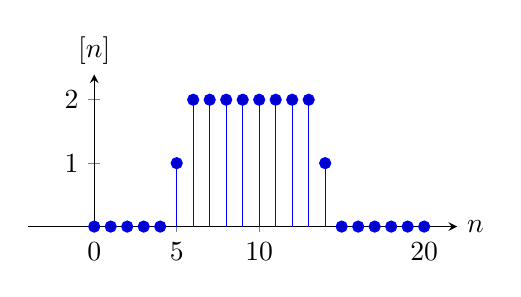
\begin{tikzpicture}
					\begin{axis} [width=200pt,height=100pt,
							axis x line=bottom,
							axis y line=middle,
							tick align=center,
							every axis x label/.style={at={(current axis.right of origin)},anchor=west},
							every axis y label/.style={at={(current axis.above origin)}, anchor=north east,above=0mm},
							xmin=-4, xmax=22,
							xtick={0, 5,10, 20},
							xlabel=$n$,
							ymin=0, ymax=2.4,
							ytick={0,...,2},
							ylabel={$\img \left[n\right]$}]
						\addplot+[ycomb] plot coordinates {(0,0) (1,0) (2,0) (3,0) (4,0) (5,1) (6,2) (7,2) (8,2) (9,2) (10,2) (11,2) (12,2) (13,2) (14,1) (15,0) (16,0) (17,0) (18,0) (19,0) (20,0)};
					\end{axis}
				\end{tikzpicture}
				\\
				\text{(b)}
				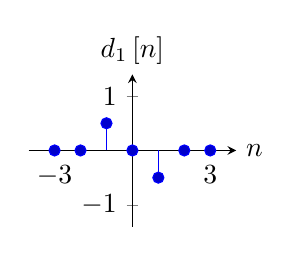
\begin{tikzpicture}
					\begin{axis} [width=120pt,height=100pt,
							axis x line=middle,
							axis y line=middle,
							tick align=center,
							every axis x label/.style={at={(current axis.right of origin)},anchor=west},
							every axis y label/.style={at={(current axis.above origin)}, anchor=north east,above=0mm},
							xmin=-4, xmax=4,
							xtick={-3,3},
							xlabel=$n$,
							ymin=-1.4, ymax=1.4,
							ytick={-1,0,1},
							ylabel={$d_1 \left[n\right]$},
							color=black]
						\addplot+[ycomb] plot coordinates {(-3,0) (-2,0) (-1,1/2) (0,0) (1,-1/2) (2,0) (3,0) };
					\end{axis}
				\end{tikzpicture}
				  &
				~
				  &
				\text{(c)}
				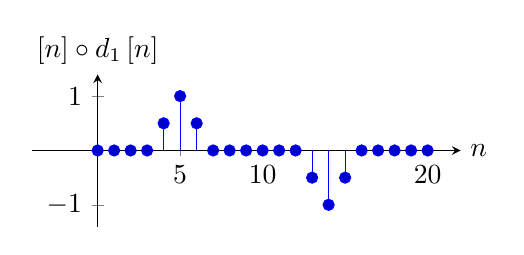
\begin{tikzpicture}
					\begin{axis} [width=200pt,height=100pt,
							axis x line=middle,
							axis y line=middle,
							tick align=center,
							every axis x label/.style={at={(current axis.right of origin)},anchor=west},
							every axis y label/.style={at={(current axis.above origin)}, anchor=north east,above=0mm},
							xmin=-4, xmax=22,
							xtick={0, 5,10, 20},
							xlabel=$n$,
							ymin=-1.4, ymax=1.4,
							ytick={-1,...,1},
							ylabel={$\img \left[n\right] \circ d_1 \left[n\right]$}]
						%\addplot+[ycomb] plot coordinates {(0,0) (1,0) (2,0) (3,0) (4,0) (5,1) (6,2) (7,2) (8,2) (9,2) (10,2) (11,2) (12,2) (13,2) (14,1) (15,0) (16,0) (17,0) (18,0) (19,0) (20,0)};
						\addplot+[ycomb] plot coordinates {(0,0) (1,0) (2,0) (3,0) (4,1/2) (5,1) (6,1/2) (7,0) (8,0) (9,0) (10,0) (11,0) (12,0) (13,-1/2) (14,-1) (15,-1/2) (16,0) (17,0) (18,0) (19,0) (20,0)};
					\end{axis}
				\end{tikzpicture}
				\\
				\text{(d)}
				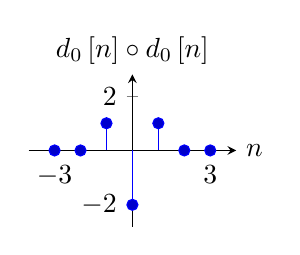
\begin{tikzpicture}
					\begin{axis} [width=120pt,height=100pt,
							axis x line=middle,
							axis y line=middle,
							tick align=center,
							every axis x label/.style={at={(current axis.right of origin)},anchor=west},
							every axis y label/.style={at={(current axis.above origin)}, anchor=north east,above=0mm},
							xmin=-4, xmax=4,
							xtick={-3,3},
							xlabel=$n$,
							ymin=-2.8, ymax=2.8,
							ytick={-2,0,2},
							ylabel={$d_0 \left[n\right] \circ d_0 \left[n\right]$},
							color=black]
						\addplot+[ycomb] plot coordinates {(-3,0) (-2,0) (-1,1) (0,-2) (1,1) (2,0) (3,0) };
					\end{axis}
				\end{tikzpicture}
				  &
				~
				  &
				\text{(e)}
				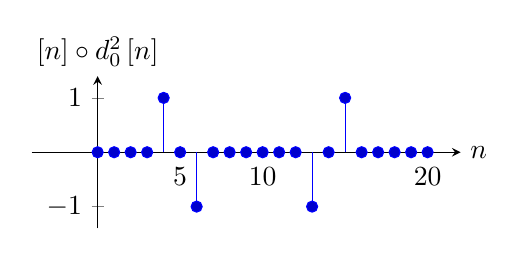
\begin{tikzpicture}
					\begin{axis} [width=200pt,height=100pt,
							axis x line=middle,
							axis y line=middle,
							tick align=center,
							every axis x label/.style={at={(current axis.right of origin)},anchor=west},
							every axis y label/.style={at={(current axis.above origin)}, anchor=north east,above=0mm},
							xmin=-4, xmax=22,
							xtick={0, 5,10, 20},
							xlabel=$n$,
							ymin=-1.4, ymax=1.4,
							ytick={-1,...,1},
							ylabel={$\img \left[n\right] \circ d_0^2 \left[n\right]$}]
						%\addplot+[ycomb] plot coordinates {(0,0) (1,0) (2,0) (3,0) (4,0) (5,1) (6,2) (7,2) (8,2) (9,2) (10,2) (11,2) (12,2) (13,2) (14,1) (15,0) (16,0) (17,0) (18,0) (19,0) (20,0)};
						\addplot+[ycomb] plot coordinates    {(0,0) (1,0) (2,0) (3,0) (4,1) (5,0) (6,-1) (7,0) (8,0) (9,0) (10,0) (11,0) (12,0) (13,-1) (14,0) (15,1) (16,0) (17,0) (18,0) (19,0) (20,0)};
					\end{axis}
				\end{tikzpicture}
			\end{array}
		$
	}
	\caption{Comparison between the output of a first-order derivative and the Laplacian of 1D signal. (a) Input signal. (b) Kernel $d_1$. (c) Output of the derivative, that is, convolution of (a) and (b). (d) Discrete approximation of the Laplacian. (e) Output of convolving the signal (a) with the Laplacian kernel (d).}
	\label{fig:discretelaplacian1d}
\end{figure}

Marr and Hildreth \cite{Marr80} used zero-crossings of the Laplacian output to compute edges,
\index{Zero-crossings}
but this method is not used nowadays for edge detection. Instead the Laplacian filter is widely used in a number of other image representations. It is used to build image pyramids (multiscale representations, \chap{\ref{chapter:image_pyramids}}), and to detect points of interest in images (it is the basic operator used to detect keypoints to compute SIFT descriptors \cite{Lowe04}).


\section{A Simple Model of the Early Visual System}

The Laplacian filter can also be used as a coarse approximation of the behavior of the {\bf early visual system}. When looking at the magnitude of the DFT of the Laplacian with $\sigma=1$ (\fig{\ref{fig:DFTlaplacians}}), the shape seems reminiscent of our subjective evaluation of our own visual sensitivity to spatial frequencies when we look at the Campbell and Robson chart (\fig{\ref{fig:csfchart}}). As the visual filter does not seem to cancel exactly the very low spatial frequencies as the Laplacian does, a better approximation is
\begin{equation}
	h = -\nabla^2 g  + \lambda g
	\label{eq:humanmodel}
\end{equation}
where the negative sign in front of the Laplacian helps to fit our perception better.
The kernel $h$ is the approximate impulse response of the human visual system, $\lambda$ is a small constant that is equal to the DC gain of the visual filter (here we have set up $\lambda = 2$ and $\sigma=5$). This results in the profile shown in \fig{\ref{fig:EVS_sigma5_lambda2}}.

\begin{figure}[h]
	\centerline{
		\includegraphics[width=.4\linewidth]{figures/derivatives/EVS_sigma5_lambda2.eps}}
	\caption{Kernel corresponding to \eqn{\ref{eq:humanmodel}} with $\lambda = 2$ and $\sigma=5$.}
	\label{fig:EVS_sigma5_lambda2}
\end{figure}
The first thing worth pointing out is that the Fourier transform of the impulse response shown in shown in \fig{\ref{fig:EVS_sigma5_lambda2}} has a shape that is qualitatively similar to the shape of the human contrast sensitivity function as discussed in \chap{\ref{chapter:fourier_analysis}}. Here we show again the Campbell and Robson chart, together with a radial section of the Fourier transform of $h$ from \eqn{\ref{eq:humanmodel}}:
\index{Contrast sensitivity function}

\begin{figure}[h]
	\centerline{
		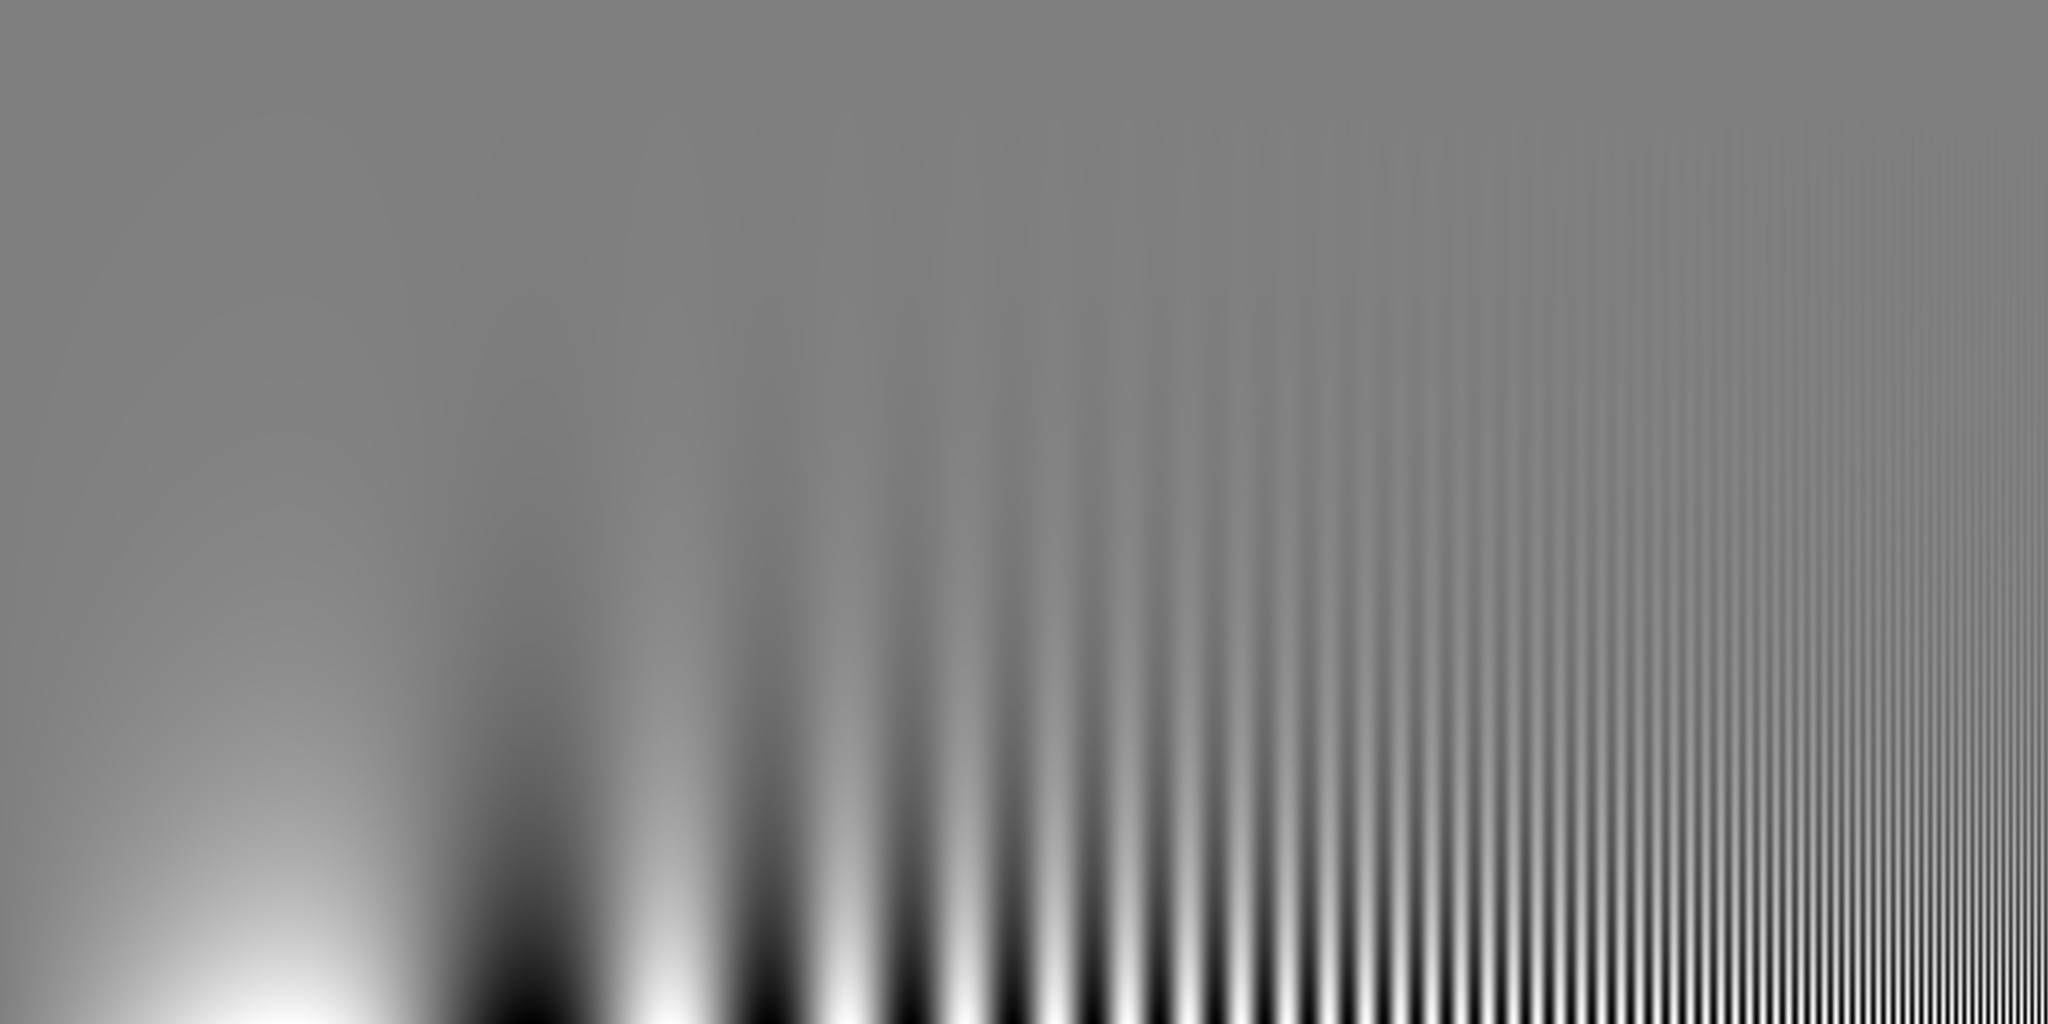
\includegraphics[trim=0cm 0cm 2cm 0cm, clip=true,width=.45\linewidth]{figures/spatial_filters/csf.jpg}
		\includegraphics[width=.45\linewidth]{figures/derivatives/dft_radial_EVS.eps}
	}
	\caption{Campbell and Robson chart, and a radial section of the Fourier transform of $h$ from \eqn{eq:humanmodel}.}
\end{figure}

This particular form of impulse response explains some visual illusions as shown in \fig{\ref{fig:vasarely}}. This visual illusion is called the {\bf Vasarely visual illusion}.
\index{Vasarely visual illusion}
Figures \ref{fig:vasarely}(a) and \ref{fig:vasarely}(d) show two grayscale pyramids  formed by superimposing squares of increasing (or decreasing) intensity. When looking at them we perceive the diagonal directions as being brighter (a) or darker (d) than their neighborhood. This is an illusion because there is not such a difference in image intensity. What mechanism is responsible of this illusion?

One explanation consists in saying that the image that we perceive is the output of a filter (as shown in \eqn{\ref{eq:humanmodel}}). Figures \ref{fig:vasarely}(b) and \ref{fig:vasarely}(e) show the output of such a filter. We can see the diagonals again as being brighter or darker but now this effect is not an illusion, the brighter and darker diagonals are really part of the filtered image. In fact, \fig{\ref{fig:vasarely}}{c} shows in blue a horizontal section at one quarter of \fig{\ref{fig:vasarely}}{b}. The red curve is the section of the input image in \fig{\ref{fig:vasarely}}{a}. We can see that the output really contains a pick in intensity on the diagonals of \fig{\ref{fig:vasarely}}{b}. The plot in \fig{\ref{fig:vasarely}}{f} shows the same for figures \ref{fig:vasarely} (d and e). For the results shown in the \fig{\ref{fig:vasarely}} we have set $\lambda = 2$ and $\sigma = 5$. The result is probably overly smooth and a more appropriate value might be around $\sigma =2$.

\begin{figure}[t]
	\centerline{
		$
			\begin{array}{ccc}
				%\text{a)}
				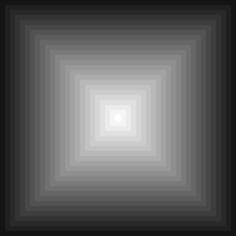
\includegraphics[width=.27\linewidth]{figures/spatial_filters/vasarely_c.jpg}
				           &
				%\text{b)}
				
\includegraphics[width=.27\linewidth]{figures/spatial_filters/vasarely_d.jpg}
				           &
				%\text{c)}
				\includegraphics[width=.27\linewidth]{figures/spatial_filters/vasarely_section.eps}
				\\
				\text{(a)} & \text{(b)} & \text{(c)}
				\\
				%\text{d)}
				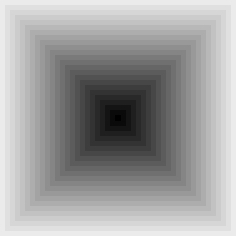
\includegraphics[width=.27\linewidth]{figures/spatial_filters/vasarely_a.jpg}
				           &
				%\text{e)}
				
\includegraphics[width=.27\linewidth]{figures/spatial_filters/vasarely_b.jpg}
				           &
				%\text{f)}
				\includegraphics[width=.27\linewidth]{figures/spatial_filters/vasarely_section_b.eps}
				\\
				\text{(d)} & \text{(e)} & \text{(f)}
			\end{array}
		$
	}
	\caption{Vasarely visual illusion. Images (a) and (d), formed by nested-squares, appear as having bright diagonals in (a) and dark in (d). Images (b) and (e) show the output of the human model given by the filter from \eqn{\ref{eq:humanmodel}}.
		Plot (c) displays the intensity profiles of images (a) and (b) as horizontal sections, with image (a) represented in red and image (b) in blue. Similarly, Plot (f) represents the intensity profiles of images (d) and (e).
		%Plot (c) shows horizontal sections of the intensity profiles of images (a) and (b) in red and blue respectively. Plot (f) shows the same for images (d) and (e).
		%Plots (c) and (f) show, in blue, a horizontal section at one quarter of image (b) and (e), showing the intensity profile as a function of $x$. The red curve is the section of the corresponding input image. %We can see that the output really contains a pick in intensity on the diagonals of the input image.
	}
	\label{fig:vasarely}
\end{figure}



%FIGURE: Show Vasarely illusion (http://web.mit.edu/persci/people/adelson/publications/gazzan.dir/vasarely.html)

% https://en.wikipedia.org/wiki/Discrete_Laplace_operator


\section{Sharpening Filter}

One example of a simple but very useful filter is a {\bf sharpening filter}. The goal of a sharpening filter is to transform an image so that it appears sharper (i.e., it contains more fine details). This can be achieved by amplifying the amplitude of the high-spatial frequency content of the image. We can achieve this with a combination of filters that we have already discussed in this section.

%\begin{figure}
%\centerline{
%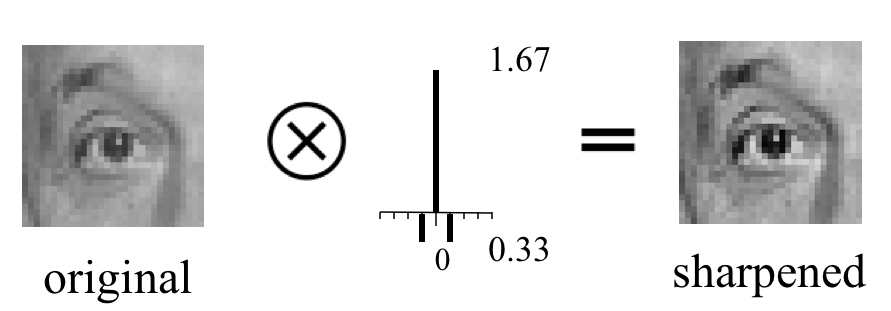
\includegraphics[width=1\linewidth]{figures/intro_signals/sharpened.jpg}}
%\caption{ Sharpening achieved by subtraction of blurred
%  components (the three filter taps of amplitude $\frac{1}{3}$) from
%  the full image (scaled appropriately). 
%} 
%\label{fig:convExamps3}
%\end{figure}


A simple way to design a sharpening filter is
to de-emphasize the blurry components of an image.  By the linearity
of the convolution operator, we're allowed to add and
subtract kernels to make a new kernel that would give us the same
filtered image as if we had added and subtracted the filtered outputs
of each of the component kernels.  For this example, we start with
twice the original image (sharp plus blurred parts), then subtract
away  the blurred components of the image:
\begin{equation}
	\text{sharpening filter} =
	\begin{bmatrix}
		0 & 0 & 0 \\
		0 & 2 & 0 \\
		0 & 0 & 0
	\end{bmatrix}
	-
	\frac{1}{16}
	\begin{bmatrix}
		1 & 2 & 1 \\
		2 & 4 & 2 \\
		1 & 2 & 1
	\end{bmatrix}
	\label{eq:sharpening}
\end{equation}
Note that the DC gain of this sharpening filter is 1. That would leave
one original image in there, plus an additional component of the sharp
details.  The perceptual result is that of a sharpened image (\fig{\ref{fig:convExamps3}}). We can apply this filter successively in order to further enhance the image details. If too much sharpening is applied we might end up enhancing noise and introducing image artifacts.


\begin{figure}
	$
		\begin{array}{ccc}
			\text{(a)}
			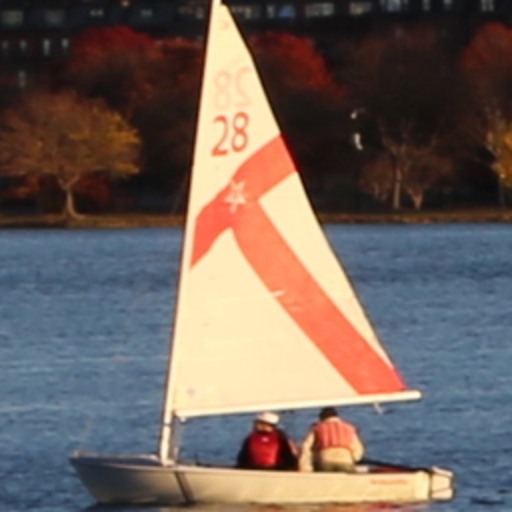
\includegraphics[width=.27\linewidth]{figures/spatial_filters/boat_sharp.jpg}
			 &
			\text{(b)}
			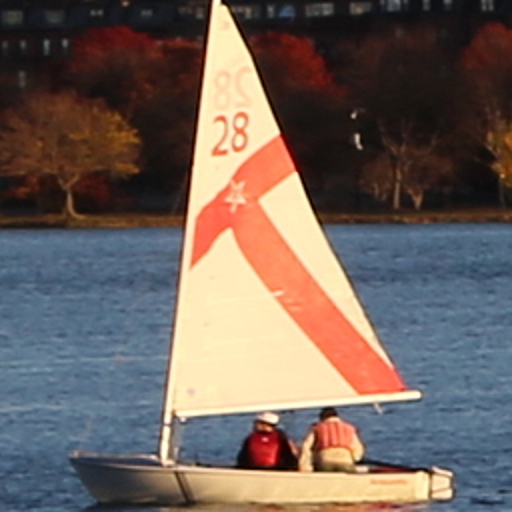
\includegraphics[width=.27\linewidth]{figures/spatial_filters/boat_sharp0.jpg}
			 &
			\text{(c)}
			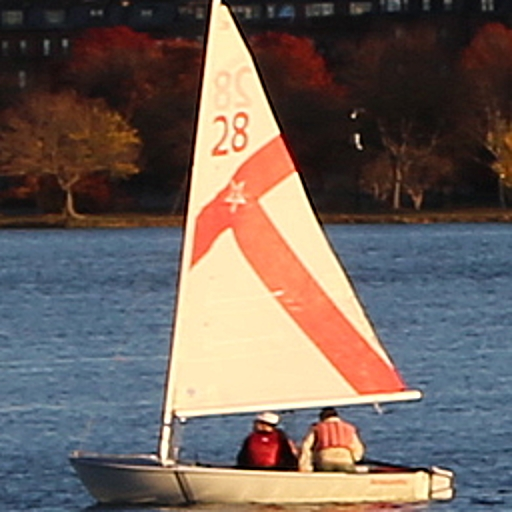
\includegraphics[width=.27\linewidth]{figures/spatial_filters/boat_sharp1.jpg}
			\\
			\text{(d)}
			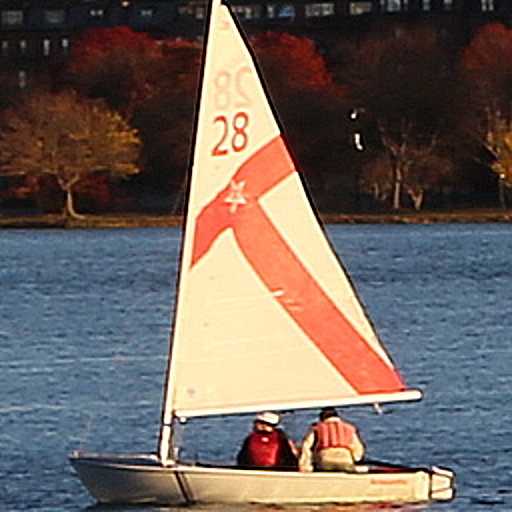
\includegraphics[width=.27\linewidth]{figures/spatial_filters/boat_sharp2.jpg}
			 &
			\text{(e)}
			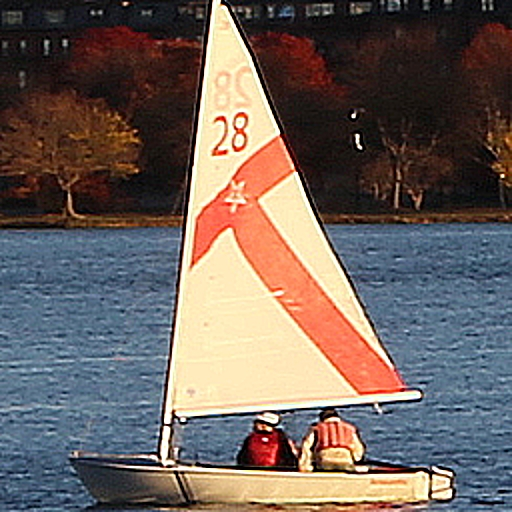
\includegraphics[width=.27\linewidth]{figures/spatial_filters/boat_sharp3.jpg}
			 &
			\text{(f)}
			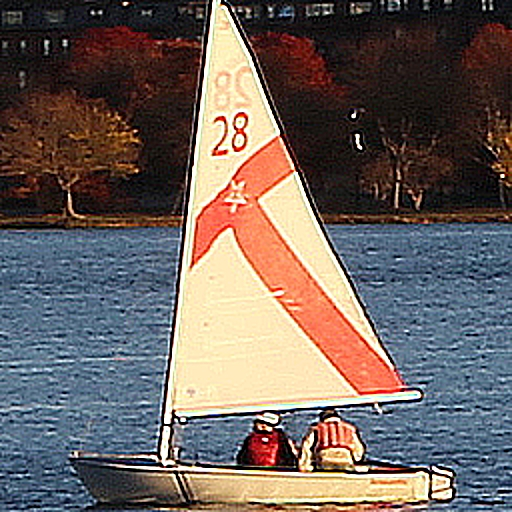
\includegraphics[width=.27\linewidth]{figures/spatial_filters/boat_sharp4.jpg}
		\end{array}
	$
	\caption{Sharpening achieved by subtraction of blurred components. (a) Original image. (b) Sharpened once by filtering with kernel from \eqn{\ref{eq:sharpening}}.  Each color channel is filtered independently. (c-f) The same filter is applied successively to the previous output. In the last image the sharpening filter has been applied five times to the input image. The last image looks substantially sharper than the original image, but close inspection will reveal some artifacts.}
	\label{fig:convExamps3}
\end{figure}


Note that the sharpening filter described here does not introduce new fine image details, it only enhances the ones already present in the image.

It is also interesting to note that this sharpening filter is very similar to the model of the early visual system that we described before.


\section{Retinex}


How do you tell gray from white? This might seem like a simple question, but one remarkable aspect of vision is that perception of the simplest quantity might be far from trivial. As a final example to illustrate the power of using image derivatives as an image representation, we will discuss here a partial answer to this question.


To understand that answering this question is not trivial, let's consider the structure of light that reaches the eye, which is the input upon which our visual system will try to differentiate black from white. The amount of light that reaches the eye from painted piece of paper is the result of two quantities: the amount of light reaching the piece of paper, and the reflectance of the surface (what fraction of the light is reflected back into space and what fraction is absorbed by the material).


If two patches receive the same amount of light, then we will perceive as being darker the patch that reflects less light. But what happens if we change the amount of light that reaches the scene? If we increase the amount of light projected on top of the dark patch, what will be seen now? What will happen if we have two patches on the same scene, each of them receiving different amounts of light? How does the visual system decide what white is and how does it deal with changes in the amount of light illuminating the scene? The visual system is constantly trying to estimate what the incident illumination is and what are the actual reflectances of the surfaces present in the scene.


If our goal is to estimate the shade of gray of a piece of painted paper, then the quantity that we care about is the reflectance of the surface. But, what happens if we see two patches of unknown reflectance, and each is illuminated with two different light sources of unknown identity?  How does the visual system manages to infer what the illumination and reflectances are?

%
%



Visual illusions are a way of getting to feel how our own visual system processes images. To experience how this estimation process works let's start by considering a very simple image as shown in \fig{\ref{fig:simultaneous}}.

\begin{figure}[t]
	\centerline{
		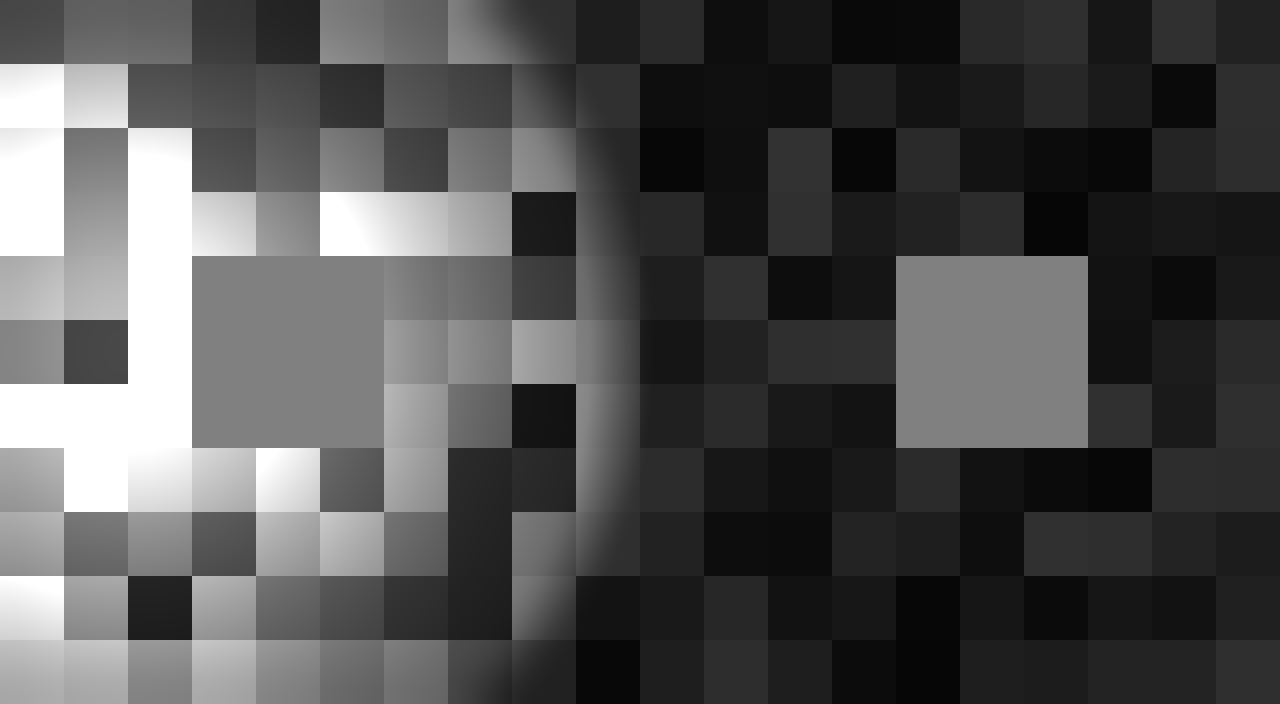
\includegraphics[width=1\linewidth]{figures/statistical_image_models/retinex.jpg}
	}
	\caption{Simultaneous contrast illusion. What happens if we see two patches of unknown reflectance, and each is illuminated with two different light sources of unknown identity?}
	\label{fig:simultaneous}
\end{figure}


This image shows a very simple scene formed by a surface with a set of squares of different gray levels illuminated by a light spot oriented toward the left. Our visual system tries to estimate the two quantities: the reflectance of each square and the illumination intensity reaching each pixel.

Let's think of the image formation process. The surface is made of patches of different reflectances $r(x,y) \in (0,1)$. Each location receives an illumination $l(x,y)$. The observed brightness is the product:
\begin{equation}
	\img (x,y) = r(x,y) \times l(x,y)
\end{equation}

Despite that what reaches the eye is the signal $\img(x,y)$, our perception is not the value of $\img(x,y)$. In fact, the squares 1 and 2 in \fig{\ref{fig:simultaneous}} have the exact same values of intensity but we see them differently which is generally explained by saying that we discount (at least partially) the effects of the illumination, $l(x,y)$.

But how can we estimate $r(x,y)$ and $l(x,y)$ by only observing $\img(x,y)$? One of the first solutions to this problem was the {\bf Retinex} algorithm proposed by Land and McCann \cite{Land1971}. Land and McCann observed that it is possible to extract $r$ and $l$ from $\img$ if one takes into account some constraints about the expected nature of the images $r$ and $l$. Land and McCann noted that if one considers two adjacent pixels inside one of the patches of uniform reflectance, the difference between the two pixel values will be very small as the illumination, even if it is nonuniform, will only produce a small change in the brightness of the two pixels. However, if the two adjacent pixels are in the boundary between two patches of different reflectances, then the intensities of these two pixels will be very different.

\marginnote{The Retinex algorithm, by Land and McCann \cite{Land1971}, is based on modeling images as if they were part of a Mondrian world (images that look like the paintings of Piet Mondrian). One example of a color Mondrian is:
	\\[6pt]
	\centerline{
		
\includegraphics[width=.4\linewidth]{figures/spatial_filters/mondrian.eps}
	}
}[-1.2in]

The Retinex algorithm
\index{Retinex algorithm}
works by first extracting $x$ and $y$ spatial derivatives of the image $\img (x,y)$ and then thresholding the gradients.  First, we transform the product into a sum using the $\log$:
\begin{equation}
	\log \img (x,y) = \log r(x,y) + \log l(x,y)
\end{equation}
Taking derivatives along $x$ and $y$ is now simple:
\begin{equation}
	\frac{\partial \log \img(x,y)}{ \partial x} = \frac{\partial \log r(x,y)}{ \partial x} + \frac{\partial \log l(x,y)}{ \partial_x}
\end{equation}
And the same thing is done for the  derivative along $y$.

Any derivative larger that the threshold is assigned to the derivative of the reflectance image $r(x,y)$ and the ones smaller than a threshold are assigned to the illumination image $l(x,y)$:

\begin{equation}
	\frac{\partial \log r(x,y)}{ \partial x} =  \left\{
	\begin{array}{rl}
		\frac{\partial \log \img (x,y)}{ \partial x} & \text{if} ~  \left| \frac{\partial \log \img (x,y)}{ \partial x} \right|>T \\
		0 ~~~~~~~~                                   & \text{otherwise}
	\end{array} \right.
\end{equation}

\Fig{\ref{fig:simultaneous2}} shows how the image derivatives are decomposed into reflectance and illumination changes.

\begin{figure}[h]
	\centerline{
		\includegraphics[width=1\linewidth]{figures/statistical_image_models/retinex_solution_b.eps}
	}
	\caption{Derivatives classified into reflectance or luminance components.}
	\label{fig:simultaneous2}
\end{figure}

Then, the image $\log r(x,y)$ is obtained by integrating the gradients, as shown in section \ref{section:editinggradientdomain}, and exponentiating the result. Finally, the illumination can be obtained as $l(x,y) = \img(x,y)/r(x,y)$. The results are shown in \fig{\ref{fig:simultaneous3}}.

\begin{figure}[h]
	\centerline{
		\includegraphics[width=1\linewidth]{figures/statistical_image_models/retinex_solution_a.eps}
	}
	\caption{Recovered components. The estimated reflectance, $r(x,y)$, is close to what we perceive. It seems that what we perceive contains part of $l(x,y)$.}
	\label{fig:simultaneous3}
\end{figure}

Note that the illumination derivatives have much lower magnitude than the reflectance derivatives; however they extend over much larger spatial regions, which means that once they are integrated, changes in brightness due to nonuniform illumination might be larger than changes due to variations in reflectance values.

Despite the simplicity of this approach it works remarkably well with images like the ones shown in \fig{\ref{fig:simultaneous}} and also with a number of real images. However, the algorithm is limited and it is easy to make it fail in situations where the visual system works, as we will see later in more depth.

The Retinex algorithm works by making assumptions about the structure of the images it tries to separate. The underlying assumption is that the illumination image, $l(x,y)$, varies smoothly and the reflectance image, $r(x,y)$, is composed of uniform regions separated by sharp boundaries. These assumptions are very restrictive and will limit the domain of applicability of such an approach. Understanding the structure of images in order to build models such as Retinex has been the focus of a large amount of research. This chapter will introduce some of the most important image models.

The recovered brightness is stronger than what we perceive. There are a number of reasons that weaken the perceived brightness. The effect is bigger if the display occupies the entire visual field. Right now the picture appears in the context of the page, which also affects our perception of the illumination. Also, the two larger squares do not seem to group well with the rest of the display, as if they were floating in a different plane. And finally, for such a simple display, the visual system does not fully separate the perception of both components.

Decomposing an image into different physical causes is known as {\bf intrinsic images decomposition}.
\index{Intrinsic images decomposition}
The intrinsic image decomposition, proposed by Barrow and Tenenbaum \cite{Barrow1978}, aims to recover intrinsic scene characteristics from images, such as occlusions, depth, surface normals, shading, reflectance, reflections, and so on.

%\subsection{Motion blur and camera shake.}

%The Gaussian filter that we have studied can be used to model how images are blur when a picture is taken out of focus, or when we remove the eyeglasses. But there are other types of image blur that also happen in natural situations.  Figure~\ref{fig:motions} shows examples of linear motion blur (fig~\ref{fig:motions}.a-c), and camera shake  (fig~\ref{fig:motions}.d-i). Motion blur happens when there are objects moving in the scene or when the camera is moving while the shutter is open. 
%Camera shake is produced due to the small camera vibration that happens while taking a picture and it is more important under low-light conditions. Camera shake can be modeled as a blur kernel, describing the camera motion during exposure, convolved with the image intensities. Depending on the shake the resulting picture looks as 

\section{Concluding Remarks}
%\reviewcomment{To be written.}

In this chapter we have covered a very powerful image representation: image derivatives (first order, second order, and the Laplacian) and their discrete approximations. Despite the simplicity of this representation, we have seen that it can be used in a number of applications such as image inpaining, separation of illumination and reflectance, and it can be used to explain simple visual illusions. It is not surprising that similar filters like the ones we have seen in this chapter emerge in convolutional neural networks when trained to solve visual tasks.

%\begin{figure}
%$
%\begin{array}{ccc}
%\text{a)}
%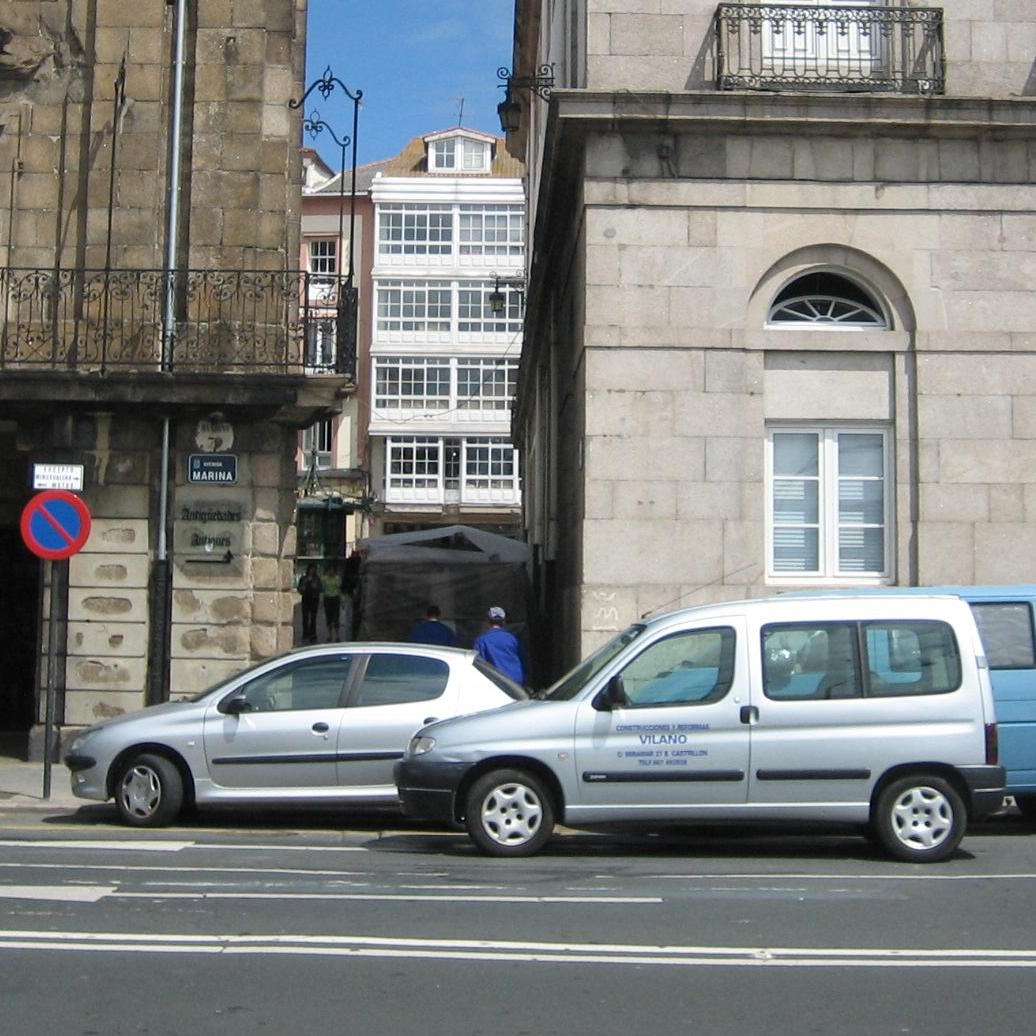
\includegraphics[width=.38\linewidth]{figures/intro_signals/street.jpg}
%&
%\text{b)}
%\includegraphics[width=.15\linewidth]{figures/intro_signals/blur_kernel2.jpg}
%&
%\text{c)}
%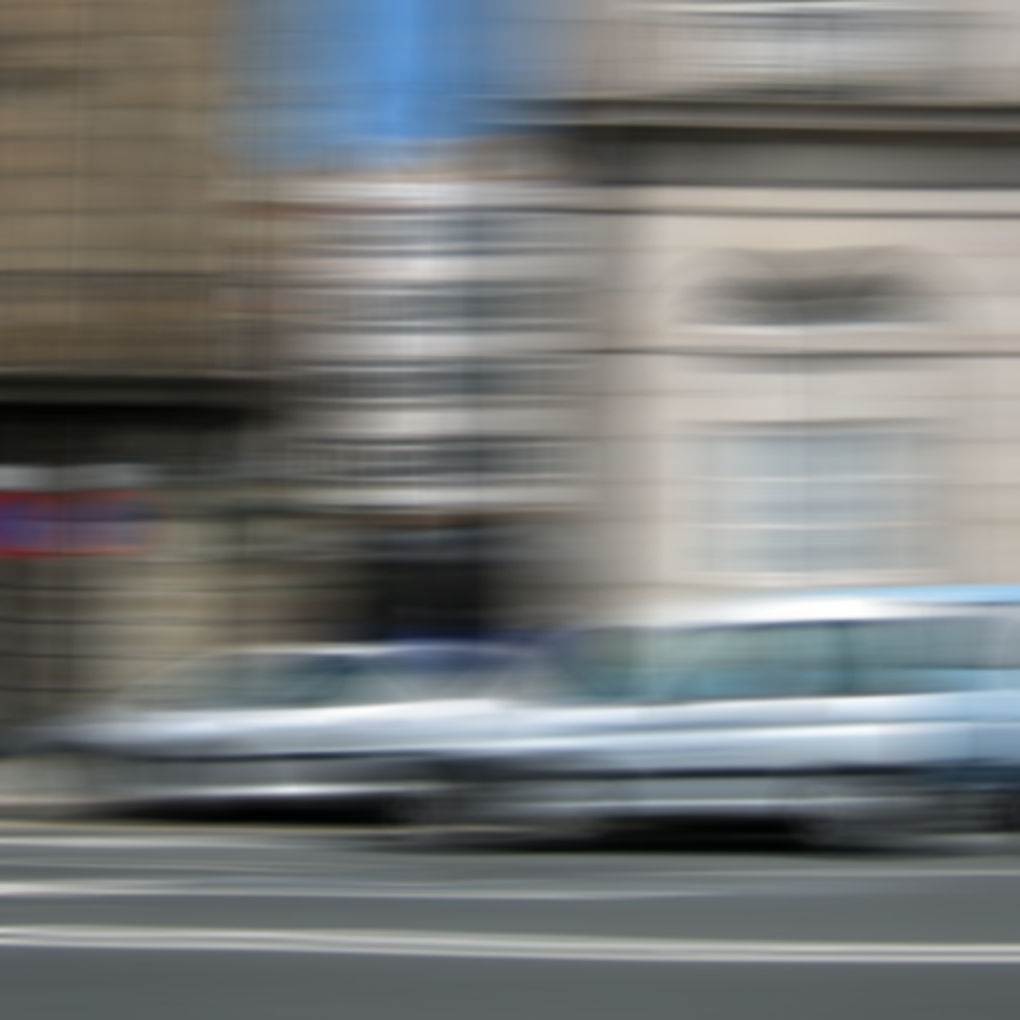
\includegraphics[width=.38\linewidth]{figures/intro_signals/street_kernel2.jpg}
%\\
%\text{d)}
%\includegraphics[width=.38\linewidth]{figures/intro_signals/bostonnight.jpg}
%&
%\text{e)}
%\includegraphics[width=.15\linewidth]{figures/intro_signals/blur_kernel5.jpg}
%&
%\text{f)}
%\includegraphics[width=.38\linewidth]{figures/intro_signals/bostonnight_kernel5.jpg}
%\\
%\text{g)}
%\includegraphics[width=.38\linewidth]{figures/intro_signals/stata.jpg}
%&
%\text{h)}
%\includegraphics[width=.15\linewidth]{figures/intro_signals/stata_blur.jpg}
%&
%\text{i)}
%\includegraphics[width=.38\linewidth]{figures/intro_signals/stata_blurry.jpg}
%\end{array}
%$
%\caption{a) Simulated motion blur, in this case it is produced because the picture is taken from a moving car. d) Simulated camera shake blur (the camera has followed a circular trajectory while the shutter was open). Probably the reader has seen this type of effect in some pictures taken at night.} 
%\label{fig:motions}
%\end{figure}

%Figure~\ref{fig:motions}.d-i shows one simulated example of camera shake. In this case, the photographer is trying to capture the scene shown in fig.~\ref{fig:motions}.d, but during exposure the camera followed a circular path. Therefore, the resulting picture (fig.~\ref{fig:motions}.f) is the convolution of the ideal picture (fig.~\ref{fig:motions}.d) with the convolution kernel (fig.~\ref{fig:motions}.e). The result has probably a familiar effect for anyone that has taken pictures at night. The light sources in the picture are like delta functions that produce multiple copies of the convolution kernel. Figure~\ref{fig:motions}.g-i shows a different example where the camera has follow a more complex trajectory.

%It will be nice to have tools capable to removing the effect of camera motion to produce sharp pictures. This is an active area of research and we will discuss approaches to this problem in chapter \ref{}.


% These are blurs that happen in nature but that are complicated even for the eye. They are convolutions but sometimes we can not write analytic functions for describing them. But they are very important. The eye can tell them apart (make a figure with the same image filtered with different blur filters) but it might have difficulties in seeing in the presence of these blurs. This is why reversing the effect of these blurs is very important and very difficult.

%Make some examples: 

% $h\left[n,m\right] = \delta \left[n-1,m\right] +  \delta \left[n+5,m-3\right]$. This filter makes the image to appear twice. This happens sometimes when taking pictures. It is not nice when a picture turns out like that and it will be nice to have tools to remove it, but reversing it is hard... Can we compute the inverse? Can we filter back the signal? We will see how to do this in a later chapter.

%
%\subsection{Artistic filters}
%
%Despite the simplicity of linear filters, they can be used to produce pleasing artistic effects. Combining linear filters with some simple non-linearities provides a very large number of possibilities. These types of image manipulation techniques are very popular as they can be implemented very efficiently and can be computed very fast even on mobile devices. Linear convolutional filters are the basis of applications such as Photoshop or Instagram. 
%
%Exploring artistic effects and playing with filters to enhance pictures is a nice way of learning and gaining intuition about linear filter theory. Figure~\ref{fig:arteffects} shows a few linear filters and the result they have in images. Those filters are easy to implement and will allow you creating nice effects.
%
%\begin{figure}
%$
%\begin{array}{ccc}
%\text{a)}
%\includegraphics[width=.38\linewidth]{figures/spatial_filters/boat.jpg}
%&
%\text{b)}
%\includegraphics[width=.15\linewidth]{figures/spatial_filters/boat_kernel.jpg}
%&
%\text{c)}
%\includegraphics[width=.38\linewidth]{figures/spatial_filters/boat_effect.jpg}
%\\
%\text{d)}
%\includegraphics[width=.38\linewidth]{figures/spatial_filters/trees.jpg}
%&
%\text{e)}
%\includegraphics[width=.15\linewidth]{figures/spatial_filters/kernel2transpose.jpg}
%&
%\text{f)}
%\includegraphics[width=.38\linewidth]{figures/spatial_filters/trees_kernel2.jpg}
%
%\end{array}
%$
%\caption{Simple linear filters can create interesting effects. a-c) Random kernel. Here, by filtering the image (a) with a random set of impulses (b) at random locations and random positive amplitudes, creates an image that seems to be drawn with a pencil (c). In this example, the image is $512 \times 512$ pixels and the kernel has a support of $64 \times 64$ pixels with 50 random dots with random amplitudes between 0.5 and 1. Each color channel is filtered independently with the same kernel. d-f) Vertical motion blur.} 
%\label{fig:arteffects}
%\end{figure}
%
%
%Intentional motion blur that can be achieved by moving the camera  while taking a picture. The example in figure~\ref{fig:arteffects}.f simulates the effect of moving the camera up and down. The linear filtering produces an interesting effect on the tree trunks making them become more visually salient while attenuating other image details. 
%
% https://ebgriffith.wordpress.com/tag/effect/

%\subsection{Bio-inspired filters}


%End-stopping

%Hubel and Viesel

%
%\section{Conclusion}
%
%%In this chapter we have talked about:
%%\begin{itemize}
%%\item Signals, images
%%\item Representations in the Space and frequency domain
%%\end{itemize}
%
%Important topics that we have not described:
%\begin{itemize}
%\item We have not gone in detail in recursive filters. Maybe we should add another example in the temporal domain?
%\item We have not described how to connect difference equations and the transfer function of a system. 
%\item We have not described how to analyze the stability of recursive systems.
%\item Feedback and feedforward systems
%\end{itemize}

% Note from antonio: Neuromorphic circuits make sense here as a first application of all the tools they have seen already. They do not need to understand quadrature or pyramids in order to understand this section.

%\input{neuro}

